\documentclass[12pt,twoside]{article}
%% \usepackage{healpix,psfig,html,graphicx,htmllist,makeidx,color,apalike} %heqn
%\usepackage{xr-hyper,healpix,html,graphicx,makeidx,color,apalike} %heqn
\usepackage{xr-hyper,healpix,html,graphicx,makeidx,color,natbib} %heqn
%\usepackage{healpix,html,graphicx,makeidx,color,natbib} %heqn
%%\usepackage{healpix,html,graphicx,makeidx,color,apalike,heqn}
%\newif\ifpdf\ifx\pdfoutput\undefined\pdffalse\else\pdfoutput=1\pdftrue\fi
\begin{htmlonly}
\renewcommand{\ell}{l}
% -*- LaTeX -*-
% This LaTeX file sets the Healpix version
% as it will appear in the documentation
% implement it with: % -*- LaTeX -*-
% This LaTeX file sets the Healpix version
% as it will appear in the documentation
% implement it with: % -*- LaTeX -*-
% This LaTeX file sets the Healpix version
% as it will appear in the documentation
% implement it with: \input{hpxversion}
% \newcommand{\hpxversion}{3.31}
% \newcommand{\hpxverstex}{3\_31}
% \newcommand{\hpxversion}{3.40}
% \newcommand{\hpxverstex}{3\_40}
% \newcommand{\hpxversion}{3.41}
% \newcommand{\hpxverstex}{3\_41}
\newcommand{\hpxversion}{3.50}
\newcommand{\hpxverstex}{3\_50}

% \newcommand{\hpxversion}{3.31}
% \newcommand{\hpxverstex}{3\_31}
% \newcommand{\hpxversion}{3.40}
% \newcommand{\hpxverstex}{3\_40}
% \newcommand{\hpxversion}{3.41}
% \newcommand{\hpxverstex}{3\_41}
\newcommand{\hpxversion}{3.50}
\newcommand{\hpxverstex}{3\_50}

% \newcommand{\hpxversion}{3.31}
% \newcommand{\hpxverstex}{3\_31}
% \newcommand{\hpxversion}{3.40}
% \newcommand{\hpxverstex}{3\_40}
% \newcommand{\hpxversion}{3.41}
% \newcommand{\hpxverstex}{3\_41}
\newcommand{\hpxversion}{3.50}
\newcommand{\hpxverstex}{3\_50}

\end{htmlonly}

\hypersetup{%
	pdftitle={HEALPix Introduction},%
	pdfauthor={HEALPix collaboration},%
	pdfkeywords={HEALPix, Introduction, Properties, Conventions},%
	colorlinks=true,
	citecolor=[rgb]{0.0,0.7,0.0},
	pagebackref=true}

%\newcommand{\myhtmlimage}[1]{\htmlimage{#1}}
\newcommand{\myhtmlimage}[1]{ }
\newcommand{\htmlfigwidth}{0.5\textwidth}
\renewcommand{\contentsname}{{TABLE OF CONTENTS}}
% to make sure that in html, the &=& in eqnarray appears normally,
% replace &=& with &\myequal& hereafter
\newcommand{\myequal}{=}
\begin{htmlonly}
\renewcommand{\myequal}{$=$}
\end{htmlonly}
\newcommand{\healpixwebpage}{http://healpix.sourceforge.net}

% commands for arbitrary link
\newcommand{\mylink}[2]{% \mylink{link_id}{link_text}
\latexhtml{\hyperlink{#1}{#2}}{\hyperref{#2}{}{}{#1}}}
% commands for targets 
% http://tex.stackexchange.com/questions/17057/hypertarget-seems-to-aim-a-line-too-low
\makeatletter
     \newcommand{\nop}[1]{\Hy@raisedlink{\hypertarget{#1}{}}}
\makeatother
\newcommand{\mytarget}[1]{\nop{#1}}%    \mytarget{id}
\begin{htmlonly}
 \newcommand{\mytarget}[1]{\label{#1}}
\end{htmlonly}

\newcommand{\npix}{{N_{\rm pix}}}
\newcommand{\Opix}{{\Omega_{\rm pix}}}
\newcommand{\nside}{N_{\rm side}}

\sloppy
\setcounter{secnumdepth}{10}%must be non-zero for cross-reference of Figs and Sections
\setcounter{tocdepth}{10}


% CROSS-LINK
%%%%http://tex.stackexchange.com/questions/41539/does-hyperref-work-between-two-files
%% add xr-hyper (part of hyperref) to used packages, *BEFORE* hyperref (or html)
\newcommand{\facname}{} % must be here because it is in idl.tex
\newcommand{\FACNAME}{} % must be here because it is in idl.tex
\externaldocument{install}
\externaldocument{csub}
\externaldocument{idl}
\externaldocument{facilities}
\externaldocument{subroutines}
\begin{htmlonly}
\externallabels{.}{/tmp/installlabels.pl}
\externallabels{.}{/tmp/csublabels.pl}
\externallabels{.}{/tmp/idllabels.pl}
\externallabels{.}{/tmp/facilitieslabels.pl}
\externallabels{.}{/tmp/subroutineslabels.pl}
\end{htmlonly}

\begin{document}

\title{The \healpix Primer}
\docid{An Overview of the \healpix concept.}
\docrv{Version \hpxversion}
\author{Krzysztof M.~G\'orski, Benjamin D.~Wandelt, Eric Hivon, Frode K.~Hansen,
and Anthony J. Banday}
\abstract{%
\healpix is a Hierarchical, Equal Area, and iso-Latitude Pixelation 
of the sphere  designed to support efficiently
(1) local operations on the pixel set,
(2) a hierarchical tree structure for  multi-resolution applications, and
(3) the global Fast Spherical Harmonic transform.
\healpix based mathematical software meets the challenges presented by
high resolution and large volume data sets, such as
the WMAP and Planck CMB mission products.
}
% -*- LaTeX -*-
% This LaTeX file sets the Healpix website
% as it will appear in the documentation
% implement it with: % -*- LaTeX -*-
% This LaTeX file sets the Healpix website
% as it will appear in the documentation
% implement it with: % -*- LaTeX -*-
% This LaTeX file sets the Healpix website
% as it will appear in the documentation
% implement it with: \input{hpxwebsite}
%
% DEPRECATED !!!! replaced with hpxwebsites.tex
%

%
% DEPRECATED !!!! replaced with hpxwebsites.tex
%

%
% DEPRECATED !!!! replaced with hpxwebsites.tex
%

\date{\today}

\frontpage
\tableofcontents
\newpage

\section{Introduction}

The analysis of functions on  domains with spherical topology occupies a
central place in physical science and engineering disciplines. 
This is particularly apparent in the fields of astronomy, cosmology, 
geophysics,  atomic and nuclear physics. In many cases the geometry is either
dictated by the object under study or approximate spherical symmetry can be
exploited to yield powerful perturbation methods. Practical
limits for the purely analytical study of these problems create
an urgent necessity for efficient and accurate numerical tools.

The 
simplicity of the spherical form belies the intricacy of global
analysis on the sphere. There is no known
point set which achieves the analogue of uniform sampling in Euclidean space and
allows exact and invertible discrete spherical harmonic decompositions
of arbitrary but band-limited functions. Any existing proposition of practical
schemes for the  discrete treatment of such functions 
on the sphere  introduces some (hopefully tiny) 
systematic error dependent on the global properties of
the point set. The goal is to minimise these errors and
faithfully represent deterministic functions as well as realizations of
random variates both
in configuration and Fourier space while maintaining computational efficiency.

We illustrate these points using as an example the field which is particularly 
close to the authors' hearts, Cosmic Microwave Background (CMB)
anisotropies. Here we are in the happy situation of expecting an explosion
of available data within the next decade.
The  Microwave Anisotropy Probe (MAP) (NASA) and Planck Surveyor (ESA)
missions are aiming
to provide multi-frequency, high resolution, full sky measurements of the anisotropy in
both temperature and polarization of the cosmic microwave
background radiation.
The ultimate data products of these missions ---
multiple microwave sky maps, each of which will have to comprise 
more than $\sim $ $10^6$ pixels in order to render the angular 
resolution of the instruments ---
will present serious challenges to those involved in the
analysis and scientific exploitation of the results of both surveys.
 
As we have learned while working with the {\it COBE} mission products, 
the digitised
sky map is an essential intermediate 
stage in information processing between 
the entry point of data acquisition by the 
instruments --- very large time ordered data streams,
and the final stage of astrophysical analysis --- 
typically producing a 
%$\lq$few'
'few'
 numerical values
of physical parameters of interest. 
{\it COBE}-DMR sky maps (angular resolution of $7^\circ$ (FWHM) in
three frequency bands, two channels each, 6144 pixels per map)
were considered large at the time of their release.

As for ongoing CMB maps, a whole sky CMB survey  
at the angular resolution
of $\sim 10'$ (FWHM), discretised with 
a few pixels per resolution element 
(so that the discretisation effects on the signal are  
sub-dominant with respect to the effects of instrument's angular response),
require map sizes of at least 
$\npix \sim  10^7$ pixels.
More pixels than that are needed to represent the Planck-HFI higher 
resolution channels.
This estimate, $\npix$, should be multiplied by  the number of frequency bands 
(or, indeed, by the number of individual
observing channels --- 74 in the case of Planck --- for the analysis work 
to be done before the
final coadded maps are made for each frequency band) to render 
an approximate expected
size of the already very compressed form of survey data which is
the input to the astrophysical analysis pipeline. 

It appears to us that very careful
attention ought to be given to devising  high resolution CMB map
structures which can maximally facilitate 
the forthcoming analyses of large size data sets, for the following
reasons:
\begin{itemize}
\item It is clearly very easy to end up with an estimated size of many GBy 
for the 
data objects which would be directly involved in the science extraction
part of the future CMB missions.
\item Many essential scientific questions
can only be answered by {\em global} studies of  future data sets.
\end{itemize}

This document is an introduction to the
properties of our proposed approach for a high resolution numerical
representation of  functions on the sphere
 --- the Hierarchical
Equal Area and iso-Latitude Pixelation  (\healpixns, see 
\htmladdnormallink{{\tt \healpixwebpage}}
{\healpixwebpage}), 
and the associated multi-purpose computer 
software package. 
 
\section[Discretisation of Functions on the Sphere]{Discretisation of Functions on the Sphere for 
High Resolution Applications:
a Motivation for \healpix}

Numerical analysis of functions on the sphere involves 
(1) a class of mathematical operations, whose objects are 
(2) discretised maps, i.e. quantizations of arbitrary functions 
according to a
chosen tessellation (exhaustive partition of the sphere into 
finite area elements). Hereafter we mostly specialise our discussion 
to CMB related applications of
\healpixns, 
but all our statements hold true generally for any relevant 
deterministic and random functions on the sphere.

Considering point (1):
Standard operations of numerical analysis which one might wish to
execute on the sphere include
convolutions with local and global kernels, 
Fourier analysis with spherical harmonics
and power spectrum estimation,
wavelet decomposition, nearest-neighbour searches, topological
analysis, including searches for extrema or zero-crossings, 
computing Minkowski functionals,
extraction of patches and
finite differencing for solving partial
differential equations.
Some of these operations become prohibitively slow  
if the sampling of functions on the sphere, and the related structure of 
the discrete data set, are not designed carefully. 

Regarding point (2): 
Typically, a whole sky map rendered by a CMB experiment contains 
({\it i}) signals coming from the sky,
which are by design strongly band-width limited (in the sense of 
spatial Fourier
decomposition) by the instrument's angular response 
function, and 
({\it ii}) a projection into the elements of a discrete map, or pixels,
of the observing instrument's noise; this pixel noise should be random,
and white, at least near the discretisation scale, with a band-width 
significantly exceeding that of all the signals. 

With these considerations in mind we propose the following list of 
desiderata 
for the mathematical structure of discretised full sky maps:

{\bf 1. Hierarchical structure of the data base}. This is recognised as 
essential for very large data bases, and was  postulated 
in construction
of the Quadrilateralized Spherical Cube 
(or quad-sphere, see 
\htmladdnormallink{{\tt http://space.gsfc.nasa.gov/ast\-ro/co\-be/skymap\_info.html}}
{http://space.gsfc.nasa.gov/astro/cobe/skymap_info.html}), 
which was used for the
{\it COBE} data. An  argument in favour of this 
proposition
states that the data elements  
which are nearby in a multi-dimensional configuration space 
(here, on the surface of 
a sphere), are also nearby in the tree structure of the data base, hence
the near-neighbour searches are conducted optimally in the data storage medium
or computer RAM.
This property, especially when implemented with a small number of base
resolution elements, 
facilitates various topological methods of analysis, 
and allows easy construction
of wavelet transforms on quadrilateral (and also triangular) grids. 
Figure~\ref{fig:quadtree} %\htmlonly{ (on page~\pageref{page:quadtree})} 
shows how a hierarchical partition with 
quadrilateral structure naturally allows for a binary vector indexing
of the data base.

\begin{figure}[!ht]
%% \centerline{\psfig{figure=quad_tree.eps,width=\textwidth}}
\latexhtml{%for latex
\centerline{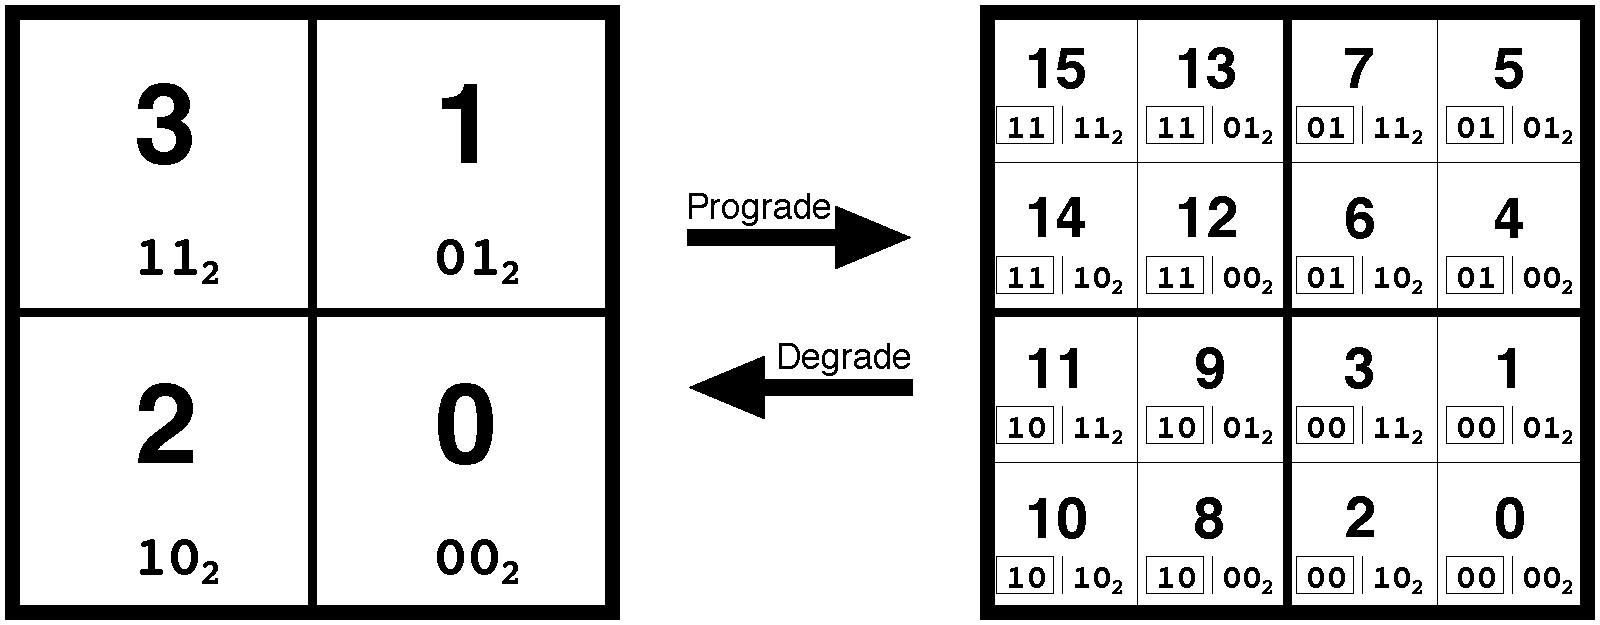
\includegraphics[width=0.9\textwidth]{fig/quad_tree.pdf}}
}{%for html
%\centerline{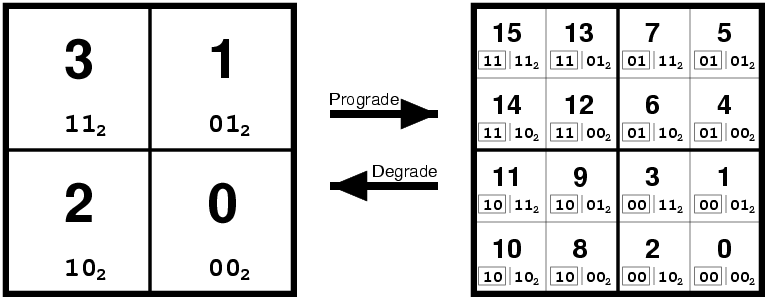
\includegraphics[bb=1pt 1pt 768pt 300pt,width=0.9\textwidth]{fig/quad_tree}\htmlimage{}}
%%%%%\centerline{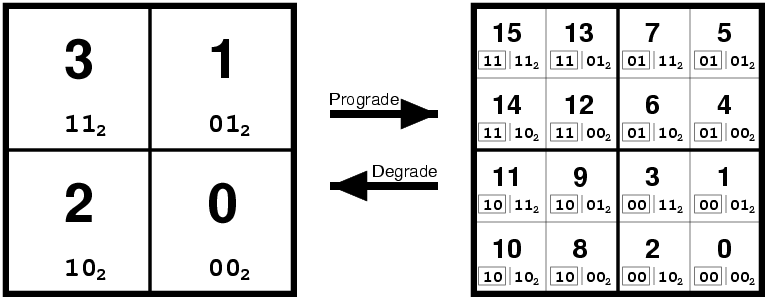
\includegraphics[width=\htmlfigwidth]{fig/quad_tree}}
\centerline{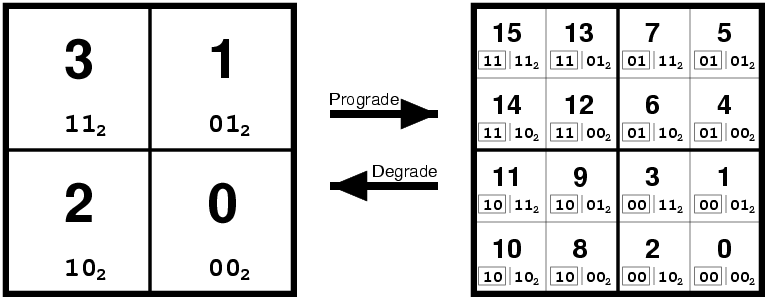
\includegraphics[width=518pt]{fig/quad_tree}}% rescaled for JPL web site -> 720 pt
}
\caption[Quadrilateral tree pixel numbering]%
{\label{fig:quadtree}%
Quadrilateral tree pixel numbering. 
The coarsely pixelated coordinate patch on
the left consists 
of four pixels. Two bits suffice to label the pixels. 
To increase the resolution, every 
pixel splits into 
4 daughter pixels shown on the right. These daughters inherit the pixel
index of their 
parent (boxed) and acquire 
two new bits to give the new pixel index. 
Several such curvilinearly mapped coordinate patches 
(12 in the case of \healpixns, and 6 in the case of the {\it COBE} quad-sphere) 
are joined at the boundaries to cover
the sphere. All pixels indices carry a prefix (here omitted for clarity) 
which identifies which base-resolution pixel they belong to.}
\end{figure}

{\bf 2. Equal areas of discrete elements of partition}. This is advantageous 
because ({\it i})
white noise generated by the  signal receiver 
gets integrated exactly into
white noise in the pixel space, and 
({\it ii}) sky signals are sampled without regional dependence, except for 
the dependence on pixel shapes, which is unavoidable with tessellations of the 
sphere. 
Hence, as much as possible given the experimental details, the pixel
size should be made sufficiently small compared to the 
instrument's resolution to avoid any excessive, and pixel shape dependent, 
signal smoothing.

{\bf 3. Iso-Latitude distribution of discrete area elements on a sphere}.  
This property
is critical for computational speed of all operations involving evaluation of 
spherical
harmonics. Since the associated Legendre polynomial components of
spherical harmonics are evaluated via
slow recursions, and 
can not be simply handled in an analogous way to the trigonometric Fast Fourier Transform, 
any deviations in the sampling grid from an iso-latitude
distribution result in a prohibitive loss of computational performance
with the growing number of sampling points, or increasing map resolution.
It is precisely this property that the {\it COBE} quad-sphere is lacking,
and this renders it impractical for applications to high resolution data.


A number of tessellations 
have been  used for discretisation and analysis 
of functions on the sphere (for example, see  
\cite{drhea},
\cite{munavi}, \cite{glesp} --- rectangular grids,
\cite{baum},  \cite{teg} --- icosahedral grids,
\cite{mathint},  \cite{crtu} ---  `igloo' grids,
and \cite{szalay}  --- a triangular grid), but none 
satisfies simultaneously all three stated requirements. 

All three requirements formulated above are satisfied by construction with the
Hierarchical Equal Area, iso-Latitude Pixelation (\healpixns) 
of the sphere, which is shown in Figure~\ref{fig:HEALPIX}.
%\htmlonly{ (on page~\pageref{page:HEALPIX}). 
A more detailed description of
\healpixns, its motivations, and applications can be found in \cite{gorskihealpix05}.

\begin{figure}[!ht]
%% \centering\mbox{\psfig{figure=introf1.ps,height=9.5cm}}
\latexhtml{%for latex
\centerline{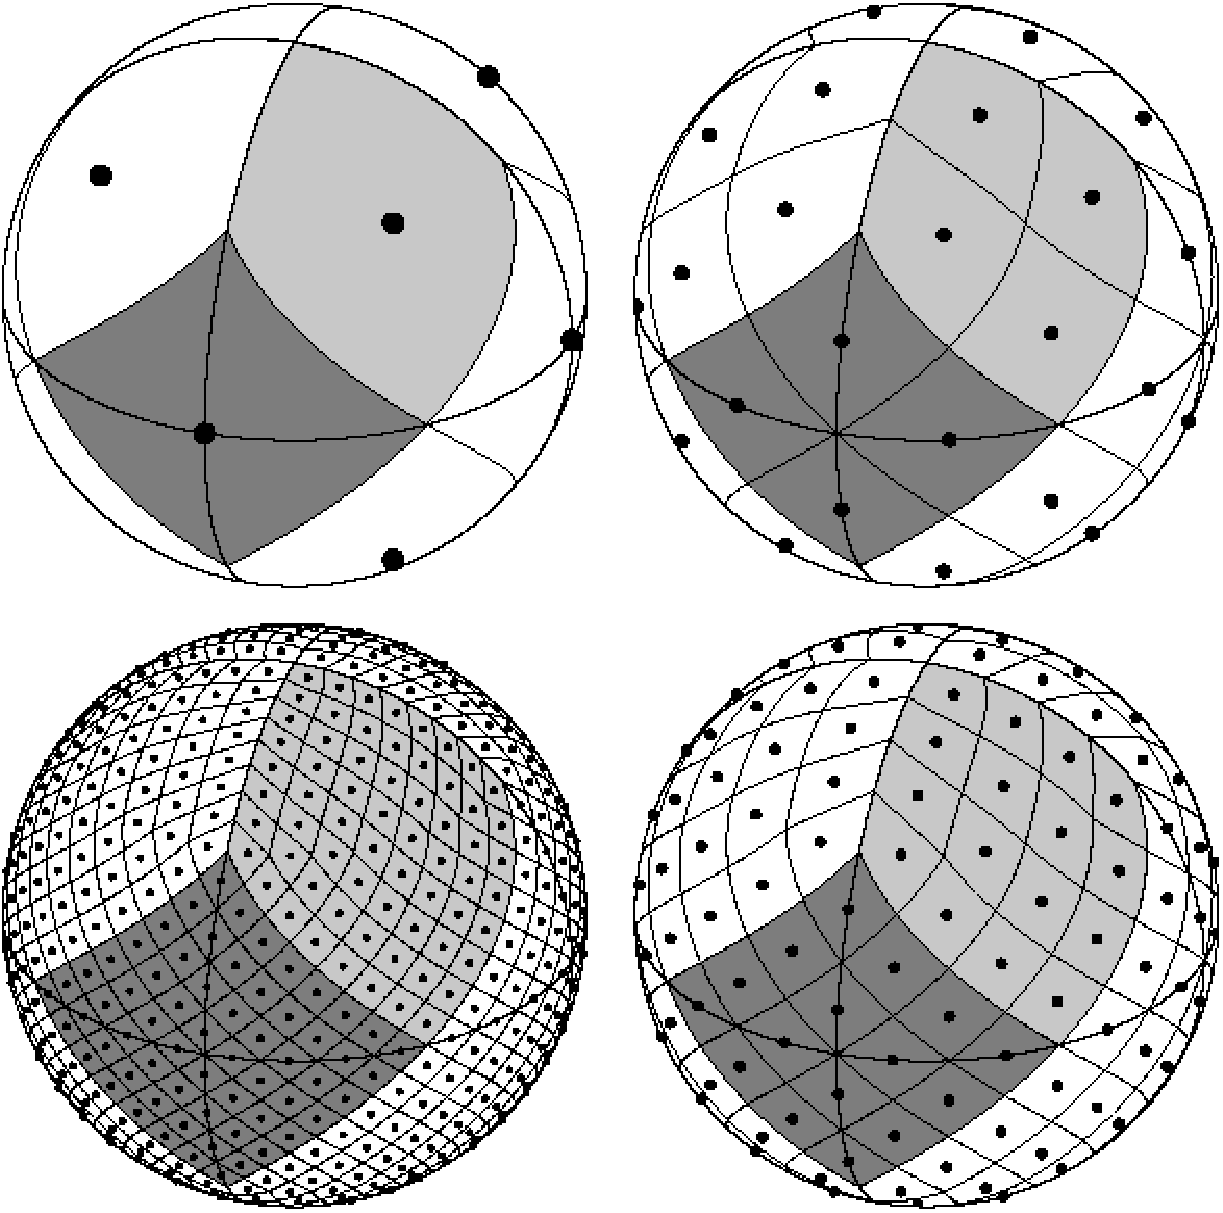
\includegraphics[height=9.5cm]{fig/introf1.pdf}}
}{%for html
%\centerline{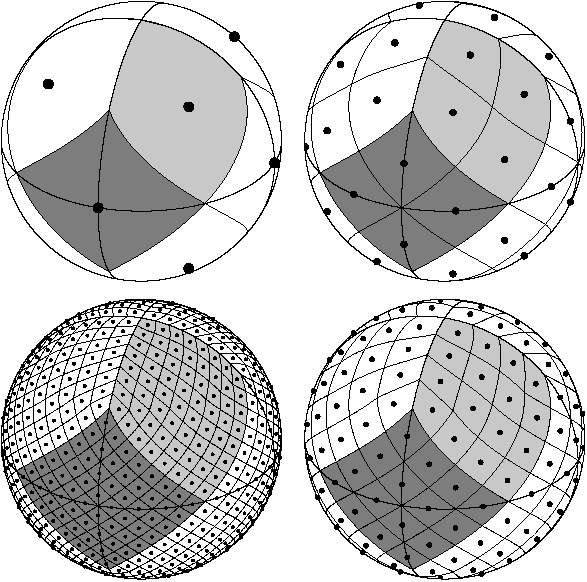
\includegraphics[bb=1pt 1pt 587pt 800pt,width=8cm]{fig/introf1}\htmlimage{}}
\centerline{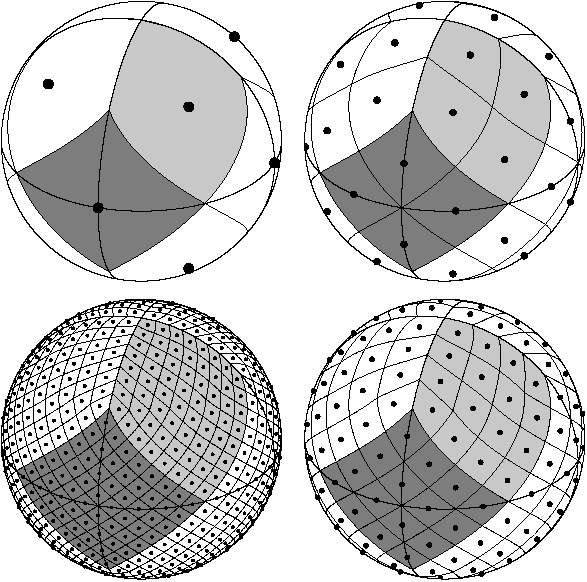
\includegraphics[width=\htmlfigwidth]{fig/introf1}}
}
\caption[Orthographic view of Healpix partition of the sphere]{%
\label{fig:HEALPIX}%
Orthographic view of \healpix partition of the sphere. 
Overplot of equator and  meridians illustrates the octahedral symmetry of  
\healpixns. 
Light-gray shading shows one of the eight (four north, and four south) 
identical polar 
base-resolution pixels. 
Dark-gray shading shows one of the four identical equatorial 
base-resolution pixels. 
Moving clockwise from the upper left 
panel the grid is hierarchically subdivided with 
the grid resolution parameter equal to 
$\nside =$ 1, 2, 4, 8, 
%$N_{\rm side} = \,1,\,2,\,4,\,8$, 
and the total number of pixels  equal to 
$\npix = 12 \times \nside^2$ = 12, 48, 192, 768. 
All pixel centers are located on $N_{\rm ring} = 4 \times \nside - 1$ rings of 
constant latitude.
Within each panel the areas of all pixels are identical.}
\end{figure}

\section{Geometric and Algebraic Properties of \healpix}

\healpix is a genuinely curvilinear partition of the sphere into exactly equal area
quadrilaterals of varying shape. The base-resolution comprises twelve pixels in three
rings around the poles and equator. 

The resolution of the grid is expressed by the parameter $\nside$ which defines the number
of divisions along the side of a base-resolution pixel that is needed to reach a desired
high-resolution partition.

All pixel centers are placed on $ 4\times \nside-1$ 
rings of constant latitude, 
and are equidistant in azimuth
(on each ring). All iso-latitude rings located between the upper and lower corners of
the equatorial base-resolution pixels, the equatorial zone, 
are divided into the same number of pixels: 
$N_{\rm eq}= 4\times \nside$. The remaining rings are located within the
polar cap regions and contain a varying number of pixels, increasing 
from ring to ring with increasing distance
from the poles by one pixel within each quadrant. 

Pixel boundaries are non-geodesic and take the very simple 
forms $\cos \theta = a \pm b \cdot \phi  $ in the equatorial zone, 
and $\cos \theta = a + b / \phi^2  $, or
  $\cos \theta = a + b / (\pi/2 - \phi) ^2  $,
%\htmlimage
in the polar caps. 
This allows one to explicitly check by simple analytical integration the 
exact area equality among pixels,
and to compute efficiently more complex objects, 
e.g. the Fourier transforms of individual pixels.


\begin{figure} [!ht]
%\centering\mbox{\psfig{figure=introf2.ps,height=14.5cm}}
\latexhtml{%for latex
\centerline{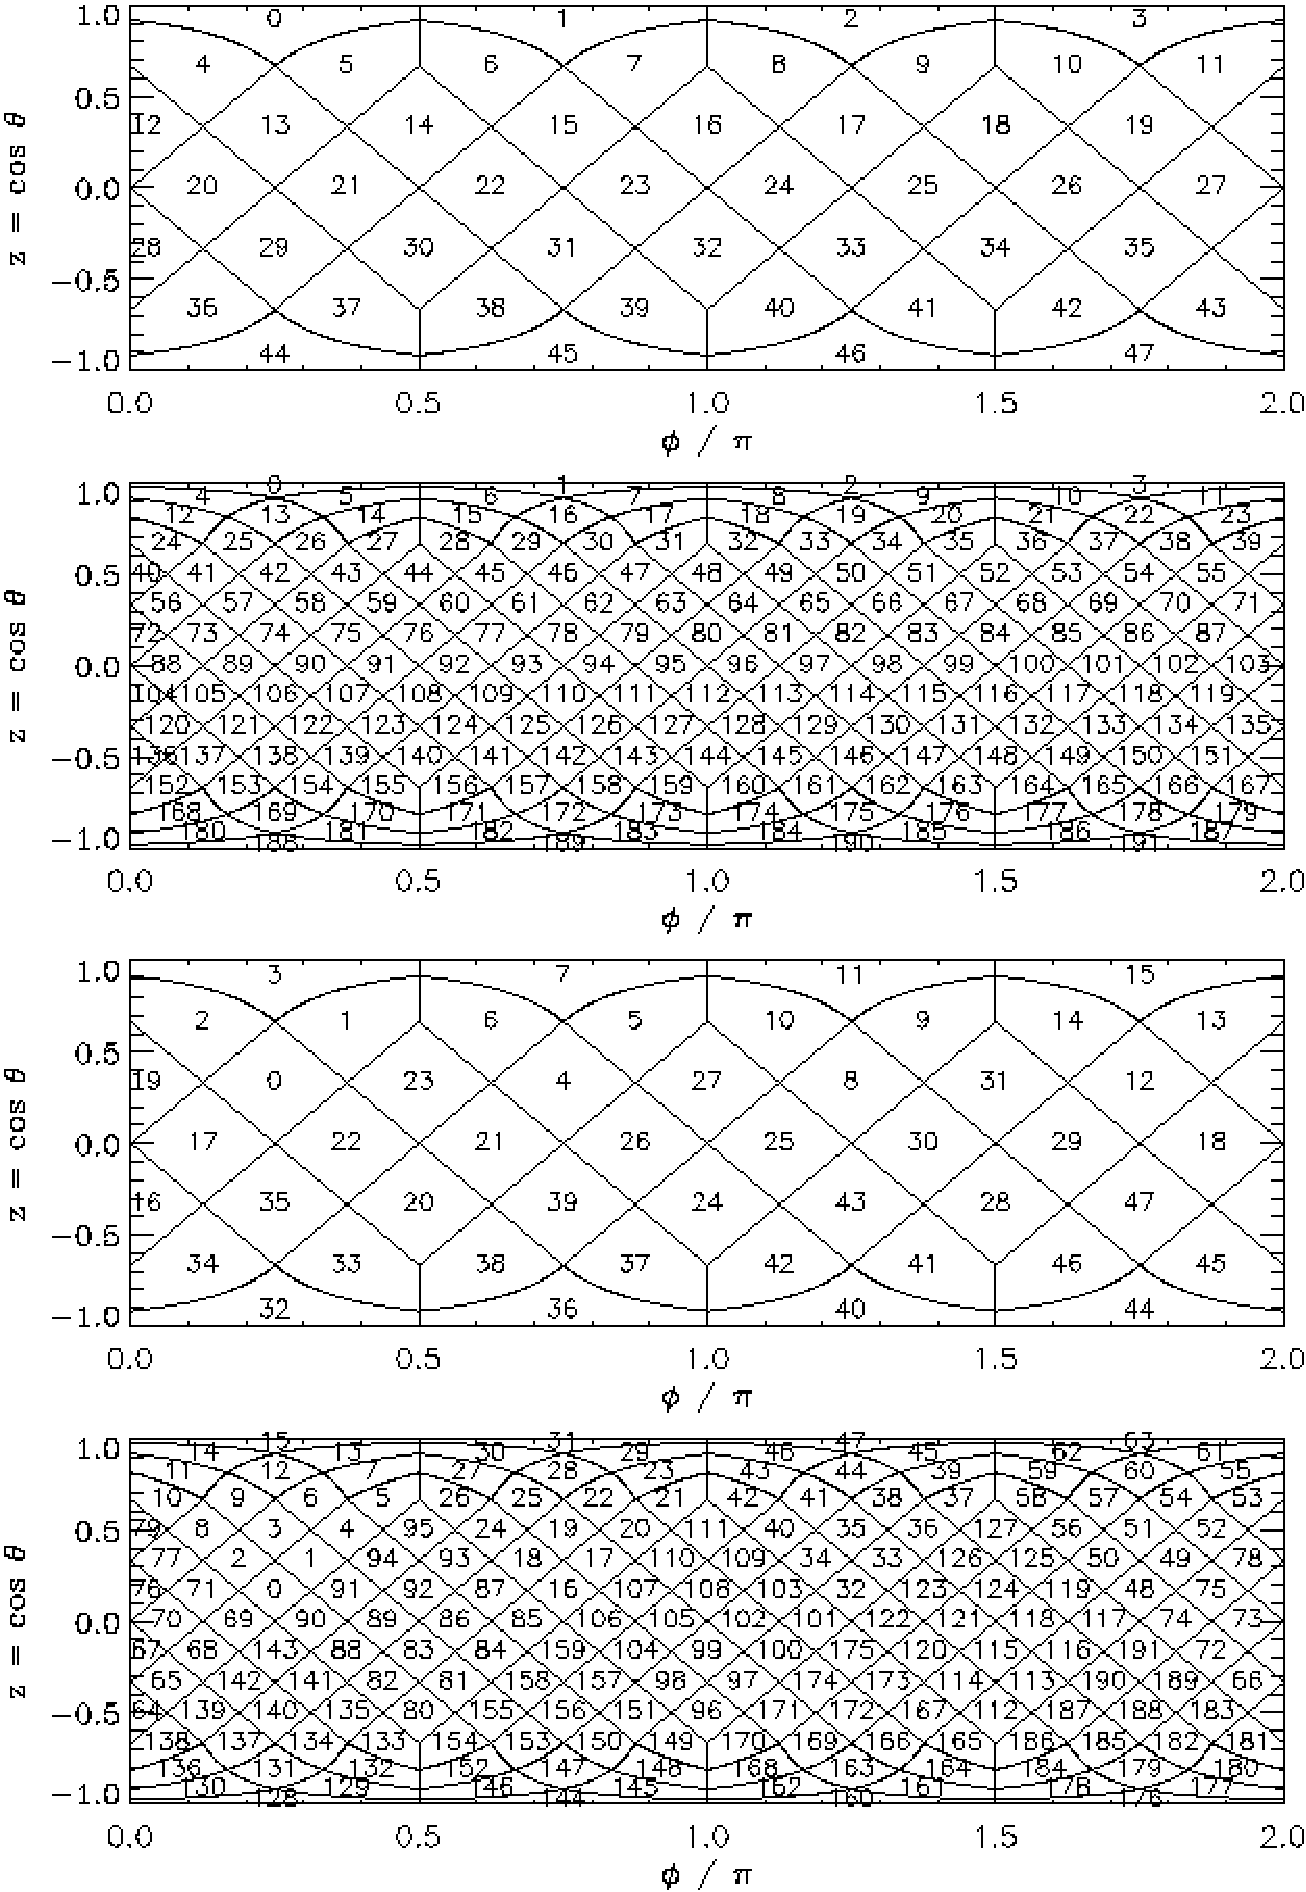
\includegraphics[height=14.5cm]{fig/introf2.pdf}}
}{%for html
%\centerline{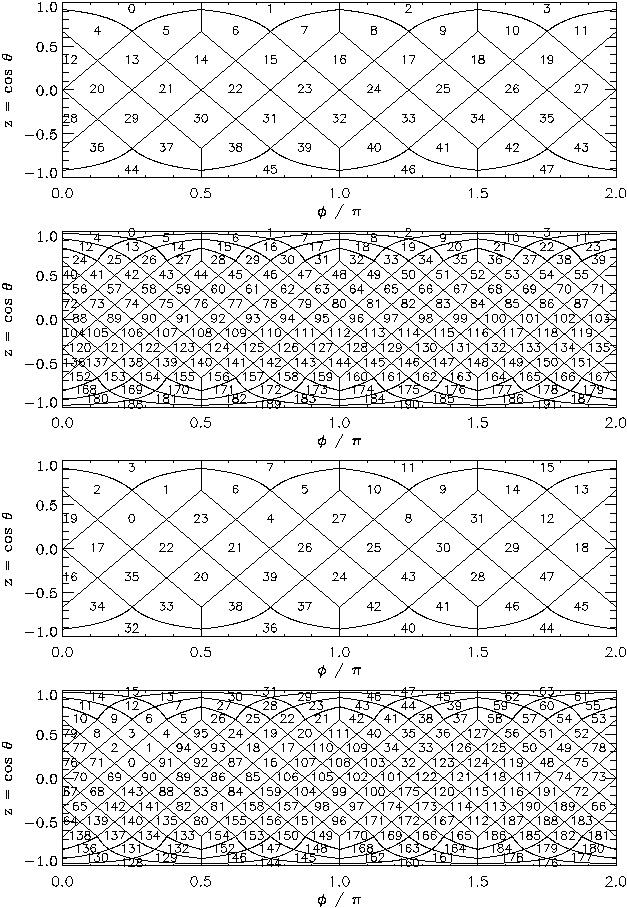
\includegraphics[bb=1pt 1pt 627pt 908pt,width=15cm]{fig/introf2}\htmlimage{}}
\centerline{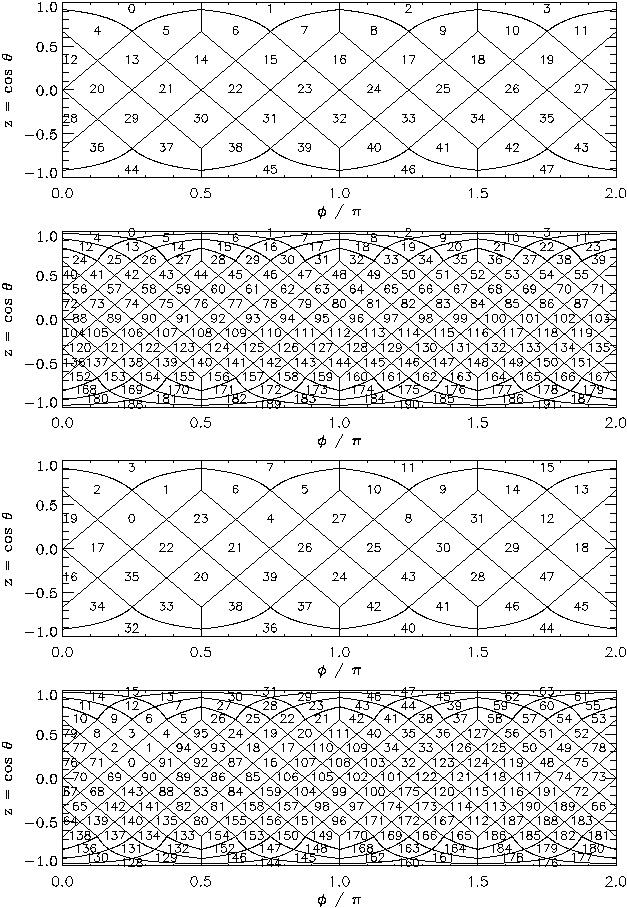
\includegraphics[width=\htmlfigwidth]{fig/introf2}}
}
\caption[Cylindrical projection]%
{\label{fig:Numbering}%
Cylindrical projection of the \healpix  division of a
sphere and two natural pixel numbering schemes (RING and NESTED) 
allowed by \healpixns. Both numbering schemes map the two dimensional 
distribution
of discrete area elements on a sphere into the one dimensional, 
integer pixel number array,
which is essential for computations involving data sets with very 
large total pixel numbers.
From top to bottom:
Panel one (resolution parameter $\nside = 2$) and panel two ($\nside = 4$)
show the RING scheme for pixel numbering, with the pixel number winding 
down from north to south pole through the consecutive isolatitude rings.
Panel three (resolution parameter $\nside = 2$) and panel four ($\nside = 4$)
show the NESTED scheme for pixel numbering within which the pixel number grows
with consecutive hierarchical subdivisions on a tree structure seeded by 
the twelve 
base-resolution pixels. 
}
\end{figure}

\subsection{RING and NESTED numbering schemes}
Specific geometrical properties allow \healpix to support two different
numbering schemes for the pixels, as illustrated in Figure~\ref{fig:Numbering}. 
% \htmlonly{on page~\pageref{page:Numbering}}.

First, in the RING scheme, 
one can simply count the pixels moving down from the north 
to the south pole along each
iso-latitude ring. It is in the RING scheme that Fourier transforms 
with spherical harmonics
are easy to implement.

Second, in the NESTED scheme, one can arrange the pixel indices 
in  twelve tree structures, corresponding to base-resolution pixels.
Each of those is organised as shown in Fig.~\ref{fig:quadtree}. %\htmlonly{on page~\pageref{page:quadtree}}.
This can easily be implemented
since, due to the simple 
description of pixel boundaries, the analytical mapping of the \healpix
base-resolution elements (curvilinear
quadrilaterals) into a [0,1]$\times$[0,1] square exists.
This tree structure allows one to implement efficiently all
applications involving  nearest-neighbour searches
\citep{whg},
and also allows for an immediate
construction of the fast Haar wavelet transform on \healpixns. 

\subsection{The Unique Identifier scheme}
\label{intro:unique}
%\mytarget{intro:unique}
As exposed above, a \healpix pixel is identified by three variables:
its numbering scheme (RING or NESTED), 
its resolution or size parameter $\nside = 2^k$ (where $k$ is a integer sometimes called 'order'),
and its index $p$ lying in $[0, 12\nside^2-1]$.
Since some applications require to process simultaneously pixels of different resolutions, it is possible
to merge the resolution $\nside$ and index $p$ into a single unique number $u$
\begin{eqnarray}
	u_{\ } &\myequal& p + 4 \nside^2, \myhtmlimage{} \label{eq:nest2uniq}
\end{eqnarray}
so that all pixels with $\nside=1$ have the unique indices 4 to 15, 
those with $\nside=2$ are in the range 16 to 63, and so on \citep{rh15}, 
thus simplifying the handling of data with heteregenous $\nside$.
Splitting the unique index $u$ into its original $\nside$ and $p$ is as simple as
\begin{eqnarray}
	\nside &\myequal& 2^{\rm{floor}\left( \log_2(u/4)/2 \right)}, \myhtmlimage{} \label{eq:ring2nest_a}\\
	     p_{\ } &\myequal& u - 4 \nside^2, \myhtmlimage{} \label{eq:ring2nest_b}
\end{eqnarray}
giving immediate access to the usual pixel based tools.

This unique indexing could in principle be applied to both the RING and NESTED schemes, 
even though the latter appears more relevant for a hierarchical description 
of data with variable resolutions: since, as noted previously, a pixel with NESTED index $p$ 
at resolution $\nside$ is subdivided in four pixels with index $4p,\, 4p+1,\, 4p+2,\, 4p+3$ 
at resolution $2\nside$, Eq.~(\ref{eq:nest2uniq}) shows that
a pixel with Nested-based unique identifier $u$ is subdivided in four smaller pixels 
whose unique identifiers are $4u,\, 4u+1,\, 4u+2,\, 4u+3$.
This Nested-based Unique identification is for instance the basis of the {\tt NUNIQ} storage scheme used for Multi-Order Coverage map (MOC) description of astronomical datasets proposed for virtual observatories \citep{moc}.

Routines implementing Eqs~(\ref{eq:nest2uniq}) and (\ref{eq:ring2nest_a}, \ref{eq:ring2nest_b}) in various languages have been available since release 3.30.


\section{The \healpix Software Package}

We have developed a package of \healpix based mathematical software, consisting
of C, C++, Fortran90, IDL/GDL, Java and Python source codes as well as documentation and
examples. Successful installation produces a set of facilities using standardised
FITS I/O interfaces 
(\htmladdnormallink{{\tt http://heasarc.gsfc.nasa.gov/docs/software/fitsio}}
{http://heasarc.gsfc.nasa.gov/docs/software/fitsio}) 
as well as 
libraries  which users can link to their own applications.
Among the tasks performed by the  components of the 
\healpix package  are the
following:

\begin{itemize}
\item Simulation of the full sky CMB temperature and polarisation maps
as realisations of random Gaussian fields, with an option to constrain
the realisation by prior information.
\item Analysis of the full sky CMB temperature and polarisation maps
resulting in power spectra and/or spherical harmonic
coefficients. Relevant conventions are given in Appendix \ref{conventions}.
{\large {\em Note that the convention used for polarization has been changed in
release 1.2!}}.
\item Global smoothing of whole sky maps with a Gaussian kernel.
\item Degradation and upgrade of the resolution of discrete maps.
\item Global searches on the maps for nearest-neighbours and 
the maxima/minima of the discretised functions.
\item Algebraic conversion of the maps between the RING and NESTED numbering
schemes, and mapping back and forth between  positions on the sphere and 
discrete pixel index space.
\item Pixel queries for various geometrical shapes (discs, triangles, polygons ...)
\item Visualisation of the \healpix formatted sky maps in the
Mollweide, orthographic, cartesian cylindrical and gnomonic
projections of the whole sky or small areas of it. 
\end{itemize}

The package includes documents which describe the installation
process, the facilities available and a large number of 
subroutines contained in the various libraries. It is
available to the scientific community  at \htmladdnormallink{{\tt
\healpixwebpage}}
{\healpixwebpage}.

\healpix was the format chosen by the {\bf WMAP}
collaboration 
for the production
of sky maps (see 
\htmladdnormallink{{\tt 
http://map.gsfc.nasa.gov/news/index.html}}{http://map.gsfc.nasa.gov/news/index.html})
 from the mission data. 

\healpix software and format have been used by the HFI and LFI consortia of {\bf Planck}
collaboration for the simulation, analysis and data release of {\bf Planck} data
(see \htmladdnormallink{{\tt
http://www.cosmos.esa.int/web/planck}}%
{http://www.cosmos.esa.int/web/planck}).

\healpix software has been selected by the GAIA satellite mission currently surveying our Galaxy
(see 
\htmladdnormallink%
{http://www.esa.int/Our\_Activities/Space\_Science/Gaia\_overview}%
{http://www.esa.int/Our_Activities/Space_Science/Gaia_overview})

% It is also being used to analyse the data provided by the balloon CMB missions
% {\bf Boomerang}
% (see \htmladdnormallink{{\tt http://cmb.PHYS.cwru.edu/boomerang/}}
% {http://cmb.PHYS.cwru.edu/boomerang/} or 
% \htmladdnormallink{{\tt http://oberon.roma1.infn.it/\-boomerang/}}
% {http://oberon.roma1.infn.it/boomerang/})
% and {\bf Archeops} (
% \htmladdnormallink{{\tt http://archeops01.free.fr/\-main\_archeops/\-index\_english.html}}
% {http://archeops01.free.fr/main_archeops/index_english.html}).

\newpage
\appendix
\section{ \healpix conventions  }
\label{conventions}%\warnhtml
A bandlimited function $f$ on the sphere can
be expanded in spherical harmonics, $Y_{\ell m}$,
as
\begin{eqnarray}
  f({ \gamma})&\myequal&\sum_{\ell =0}^{l_{max}}\sum_{m}a_{\ell m}Y_{\ell m}(\gamma),\myhtmlimage{}\label{eq:alms}
\end{eqnarray}
where ${{\gamma}}$ denotes a unit vector pointing at polar angle $\theta\in[0,\pi]$ and
azimuth $\phi\in[0,2\pi)$. Here we have assumed that there is insignificant signal power in modes
with $\ell>\ell_{max}$ and introduce the  notation that all sums over $m$ run from
$-\ell_{max}$ to $\ell_{max}$ but all quantities with index ${\ell m}$ vanish
for $m>\ell$. Our conventions for $Y_{\ell m}$ are defined in subsection
\ref{sphericalstuff} below.

Pixelating $f({ \gamma})$ corresponds to sampling it at $N_{\rm{pix}}$
 locations $\gamma_{p}$, $p\in[0,N_{\rm{pix}}-1]$. The sample
function values $f_p$ can then be used  
to estimate  $a_{\ell m}$. A straightforward estimator is
\begin{eqnarray}
  \hat{a}_{\ell m}&\myequal& \frac{4\pi}{N_{\rm{pix}}}\sum_{p=0}^{N_{\rm{pix}}-1}
  Y^\ast_{\ell m}(\gamma_p) f(\gamma_p),\myhtmlimage{}\label{eq:hata}
%  \hat{a}_{\ell m}&\myequal& \frac{4\pi}{N_{\rm{pix}}}\sum_{p=0}^{N_{\rm{pix}}-1} 
%  Y^\ast_{\ell m}(\gamma_p) f(\gamma_p),\label{eq:hata}
\end{eqnarray}
where the superscript star denotes complex  conjugation, and an equal weight was assumed for each pixel. This
zeroth order estimator, as well as  higher order  estimators, are implemented in the
Fortran90 facility \htmlref{{\tt anafast}}{fac:anafast}, included in the
package. 
%Publications discussing these estimators and the  generalised
%quadrature problem on the sphere (Hivon {\em et al.~}) are  in preparation.

% \begin{htmlonly}
% {\Large{
% \textcolor{red}{This section contains many equations that may not show up correctly in HTML.
% We recommend that the Postscript document be used instead.}
% }}
% \end{htmlonly}

\subsection{Angular power spectrum conventions}
%\warnhtml
These $\hat{a}_{\ell m}$ can be used to compute estimates of the angular power spectrum
 $\hat{C}_\ell$ as 
\begin{eqnarray}
  \hat{C}_\ell&\myequal&\frac{1}{2l +1}\sum_{m} \vert\hat{a}_{\ell m}\vert^2.\myhtmlimage{}\label{eq:hatC}
%  \hat{C}_\ell&=&\frac{1}{2l +1}\sum_{m} \vert\hat{a}_{\ell m}\vert^2.\label{eq:hatC}
\end{eqnarray}
Equations (\ref{eq:hata}) and (\ref{eq:hatC}) above do not consider the impact of a pixel masking or weighting 
$f(\gamma_p) \longrightarrow f(\gamma_p) w(\gamma_p)$ 
on the power spectrum estimation of $f$, which is described in 
\citet{whg2001}
and addressed in
\citet{master}, \citet{polspice}, \citet{xspect}, \citet{xfaster} and
\citet{planck2015-11}
among others.
% and in 
% \htmladdnormallink{http://www2.iap.fr/users/hivon/software/PolSpice/}{%
% http://www2.iap.fr/users/hivon/software/PolSpice/}

The \healpix package contains the Fortran90 facility 
\htmlref{{\tt synfast}}{fac:synfast}, 
which takes as input a power spectrum $C_\ell$ and generates a realisation of
$f(\gamma_p)$
on the \healpix grid.  The convention for power spectrum input into
{\tt synfast} is straightforward: each $C_\ell$ is just the expected
variance of the $a_{\ell m}$ at that $\ell$. 

\begin{verse}
{\bf Example}: The spherical harmonic coefficient $a_{00}$ is the
integral of the $f(\gamma)/\sqrt{4 \pi}$ over the sphere. To 
obtain realisations of functions which have $a_{00}$ distributed as a Gaussian
with zero mean and variance 1, set $C_0$ to 1.  The value of the
synthesised function at each pixel will
be Gaussian distributed with mean zero and variance $1/(4\pi)$. 
As required,  the integral of $f(\gamma)$ over the full $4\pi$
solid angle of the sphere has zero mean and variance $4\pi$. 
\end{verse}
Note that this definition implies the standard result that the total power
at the angular wavenumber $\ell$ is $(2l+1)C_\ell$, because there are
$2\ell+1$ modes for each  $\ell$. 

This defines unambiguously how the $C_\ell$ have to be defined given the
units of the physical  quantity $f$. In  cosmic
microwave background research,
popular choices for simulated maps are 
\begin{itemize}
\item $\Delta T/T $, a dimensionless quantity measuring relative
fluctuations about the average CMB temperature.
\item The absolute quantity $\Delta T$ in $\mu K$ or $K$.
\end{itemize}

\subsection{\healpix and CMBFAST}
\label{subsec:cmbfast}
A widely used  solver of the Boltzmann equations for the computation
of theoretical predictions of the spectrum of CMB anisotropy is CMBFAST
(\htmladdnormallink{{\tt http://www.physics.nyu.edu/matiasz/CMBFAST/cmbfast.html}}
{http://www.physics.nyu.edu/matiasz/CMBFAST/cmbfast.html}).

CMBFAST makes its outputs in ASCII files, which instead
of $C_{X,\ell}$ contain quantities defined as
\begin{eqnarray}
  D_{X,\ell}&\myequal&\frac{l(l+1)}{(2\pi)T_{CMB}^2}C_{X,\ell},\myhtmlimage{}
\end{eqnarray}
where $T_{CMB}=2.726K$ is the temperature of the CMB today and $X$ stands for T,
E, B or C (see \S~\ref{subsec:pol}).  

The version 4.0 of CMBFAST also created a FITS file containing the power spectra
$C_{X,\ell}$, designed for interface with \healpix. The spectra for polarization were renormalized to match the
normalization used in \healpix~1.1, which was different from the one used by
CMBFAST and by \healpix~1.2 (see \S~\ref{subsub:relatoldversion} for details).

% Since \healpix 1.2 now uses the same normalization as CMBFAST, 
% we provide a new version of the file {\tt fitsout.f} used by CMBFAST, so that
% it creates FITS files with the same normalization as the rest of the code. 

The newer version of CMBFAST (4.2, released in Feb. 2003) will generate FITS files containing
$C_{X,\ell}$, with the same convention for polarization as the one used
internally. It will therefore match the convention adopted by \healpix in its
version 1.2.

For backward compatibility, we provide an IDL code 
(\htmlref{{\tt convert\_oldhpx2cmbfast}}{idl:convert_oldhpx2cmbfast}) 
to change the normalization of existing FITS files created with CMBFAST 4.0. 
When created with the correct normalization (with CMBFAST 4.2)
or set to the correct normalization (using {\tt convert\_oldhpx2cmbfast}), the FITS file will include a
specific keyword ({\tt POLNORM = CMBFAST}) in their header to identify them.
The map simulation code 
\htmlref{{\tt synfast}}{fac:synfast}
will issue a warning if the input power
spectrum file does not contain the keyword {\tt POLNORM}, but no attempt will
be made to renormalize the power spectrum. If the keyword is present, it will be
inherited by the simulated map.

% Future
% versions of CMBFAST are planned to output \healpix compatible power
% spectrum predictions already in FITS format. Once this new version is
% available, a WWW page, linked to from both the CMBFAST and \healpix
% WWW--sites, will be made available describing the combined 
% usage of the two packages.


\subsection{Polarisation convention}
\label{subsec:pol}
\newcommand{\Cl}[1]{C_{\ell}^{\rm #1}}
\newcommand{\Chl}[1]{C_{\ell}^{\rm{#1}}}
\newcommand{\Czl}[1]{C_{\rm{#1},\ell}}
\newcommand{\alm}[1]{a_{\ell m}^{\rm #1}}
\newcommand{\azlm}[1]{a_{{\rm #1},\ell m}}
\newcommand{\pushup}{\rule[.3cm]{0cm}{.2cm}}
\newcommand{\pushdn}{\rule[-.3cm]{0cm}{.2cm}}
\newcommand{\push}{\pushup\pushdn}
\newcommand{\vecn}{{\bf n}}
\newcommand{\veceo}{{\bf{e}_{1}}}
\newcommand{\vecet}{{\bf{e}_{2}}}
\newcommand{\vectheta}{{\bf{e}_\theta}}
\newcommand{\vecphi}{{\bf{e}_\phi}}
\newcommand{\mattwo}[2]
{{
\left( 
\begin{array}{c} #1 \push \\#2 \push \end{array}
\right) 
}}

\begin{figure}[!ht]
%% \psfig{file=plot_orthpol.ps,width=5in,angle={90}}
%% \includegraphics[bb=113pt 27pt 573pt 764pt, angle=90,width=5in,clip]{plot_orthpol}
\latexhtml{%for latex
\centerline{\includegraphics[angle=90, bb=120pt 1pt 600pt 800pt, width=\textwidth,clip]{fig/plot_orthpol.pdf}}
}{%for html
%% \centerline{\includegraphics[bb=1pt 1pt 460pt 737pt,width=5in,angle=90]{fig/plot_orthpol}\htmlimage{}}
%\centerline{\includegraphics[bb=1pt 1pt 800pt 792pt,width=6in]{fig/plot_orthpol2}\htmlimage{}}
%%%%%\centerline{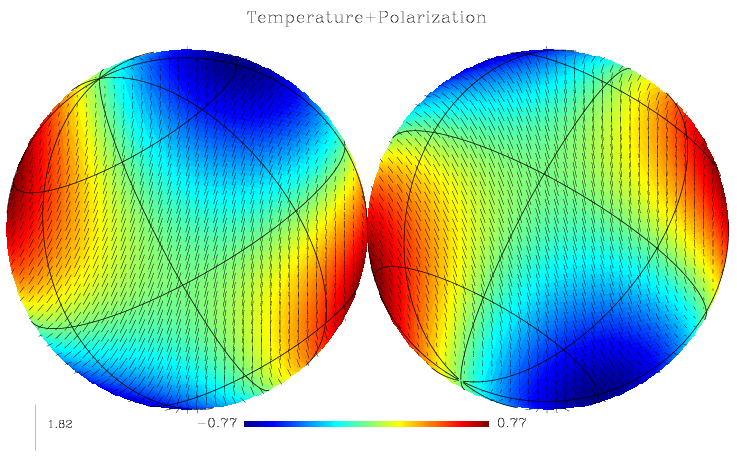
\includegraphics[width=\htmlfigwidth]{fig/plot_orthpolrot}}
\centerline{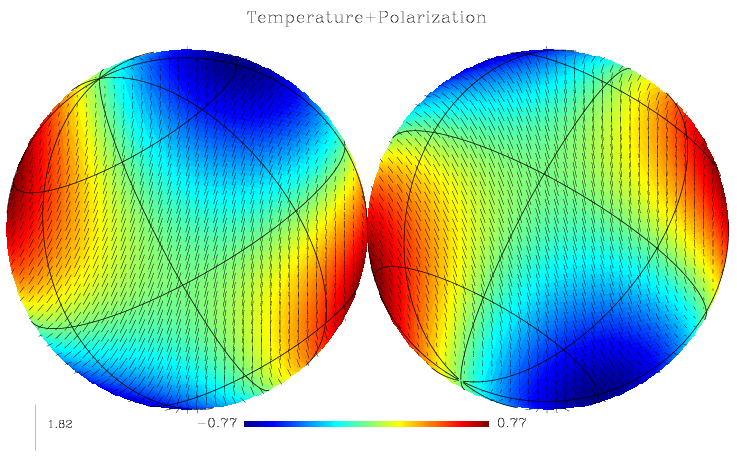
\includegraphics[width=520pt]{fig/plot_orthpolrot}} % rescaled for JPL web site -> 720
}
\caption[T and P]%
{\label{fig:orthpol}%
Orthographic projection of a fake full sky for temperature (color
coded) and polarization (represented by the rods). All the input Spherical
Harmonics coefficients are set to 0, except for
$a_{21}^{TEMP}=\ -\ a_{2-1}^{TEMP}=1$ and
$a_{21}^{GRAD}=\ -\ a_{2-1}^{GRAD}=1$}
\end{figure}

\subsubsection{Internal convention}
%\warnhtml
Starting with version 1.20 (released in Feb 2003),\healpix uses the same
conventions as CMBFAST for the sign and normalization of the polarization power
spectra, as exposed below (adapted from \cite{zalda}). How this relates to
what was used in previous releases is exposed in~\ref{subsub:relatoldversion}.

\begin{quotation}
\footnotesize
The CMB radiation field is described by a $2\, \times \, 2$ 
intensity tensor
$I_{ij}$
\citep{chandra}. The Stokes parameters $Q$ and $U$ are defined as 
$Q=(I_{11}-I_{22})/4$ and $U=I_{12}/2$, while the temperature anisotropy 
is given by $T=(I_{11}+I_{22})/4$. The fourth Stokes parameter $V$ that
describes circular polarization is not necessary in standard cosmological 
models because it cannot be generated through the process of Thomson 
scattering. While the temperature is a scalar quantity $Q$ and $U$ are
not. They depend on the direction of observation $\vecn$
and on the two axis $(\veceo, \vecet)$ 
perpendicular to $\vecn$ used to define them. If for a given 
$\vecn$ the axes $(\veceo, \vecet)$ are rotated by an angle
$\psi$ such that 
${\veceo}^{\prime}=\cos \psi \ {\veceo}+\sin\psi \ {\vecet}\myhtmlimage{}$ 
and ${\vecet}^{\prime}=-\sin \psi \ {\veceo}+\cos\psi \ {\vecet}\myhtmlimage{}$
the Stokes parameters change as
\begin{eqnarray}
  Q^{\prime}&\myequal&\cos 2\psi \  Q + \sin 2\psi \ U \nonumber \myhtmlimage{} \\  
  U^{\prime}&\myequal&-\sin 2\psi \ Q + \cos 2\psi \ U     \myhtmlimage{}  \label{QUtrans} 
\end{eqnarray}

To analyze the CMB temperature on the sky, it is natural to
expand it in spherical harmonics. These are not appropriate 
for polarization, because   
the two combinations $Q\pm iU$ are quantities of spin $\pm 2$
\citep{goldberg}. They 
should be expanded in spin-weighted harmonics $\, _{\pm2}Y_l^m$ 
\citep{spinlong, longspin},
\begin{eqnarray}
  T(\vecn)&\myequal&\sum_{lm} a_{T,lm} Y_{lm}(\vecn) \nonumber \\
  (Q+iU)({\bf n})&\myequal&\sum_{lm} 
  a_{2,lm}\;_2Y_{lm}({\bf n}) \nonumber \myhtmlimage{} \\
  (Q-iU)({\bf n})&\myequal&\sum_{lm}
  a_{-2,lm}\;_{-2}Y_{lm}({\bf n}).
  \myhtmlimage{}   \label{Pexpansion}
\end{eqnarray}
To perform this expansion, $Q$ and $U$ in equation (\ref{Pexpansion})
are measured relative to $(\veceo, \vecet)=(\vectheta, \vecphi)$, the unit vectors of the spherical coordinate system.
Where $\vectheta$ is tangent to the local meridian and directed from North
to South, and $\vecphi$ is tangent to the local parallel, and directed from
West to East.
The coefficients $_{\pm 2}a_{lm}$ 
are observable on the sky and their power spectra
can be 
predicted for different cosmological models. Instead of $_{\pm 2}a_{lm}$
it is convenient
to use their linear combinations
\begin{eqnarray}
a_{E,lm}&\myequal&-(a_{2,lm}+a_{-2,lm})/2  \nonumber \myhtmlimage{} \\
a_{B,lm}&\myequal&-(a_{2,lm}-a_{-2,lm})/2i, \myhtmlimage{}
\end{eqnarray}
which transform differently 
under parity.
Four power spectra are needed to
characterize fluctuations in a gaussian theory,
the autocorrelation between 
$T$, $E$ and $B$ and the cross correlation of $E$ and $T$.
Because of parity considerations the cross-correlations
between $B$ and the
other quantities vanish and one is left with
\begin{eqnarray}
  \langle a_{X,lm}^{*}
  a_{X,lm^\prime}\rangle &\myequal& \delta_{m,m^\prime}C_{Xl}
  \quad
  \langle a_{T,lm}^{*}a_{E,lm}\rangle=\delta_{m,m^\prime}C_{Cl},\myhtmlimage{}\label{Cls} 
\end{eqnarray}
where
$X$ stands for $T$, $E$ or $B$, $\langle\cdots \rangle$
means ensemble average and $\delta_{i,j}$ is the Kronecker delta.  

We can rewrite 
equation (\ref{Pexpansion}) as
\begin{eqnarray}
 T({\bf n})&\myequal&\sum_{lm} a_{T,lm} Y_{lm}(\vecn) \nonumber \\
 Q({\bf n})&\myequal&-\sum_{lm} a_{E,lm} X_{1,lm} 
   +i a_{B,lm}X_{2,lm} \nonumber \\
 U({\bf n})&\myequal&-\sum_{lm} a_{B,lm} X_{1,lm}-i a_{E,lm} X_{2,lm}
 \myhtmlimage{}
 \label{Pexpansion2}
\end{eqnarray}
where we have introduced
$X_{1,lm}({\bf n})=(\;_2Y_{lm}+\;_{-2}Y_{lm})/2$
and $X_{2,lm}({\bf n})=(\;_2Y_{lm}-\;_{-2}Y_{lm})/ 2$.
They satisfy $Y^{*}_{lm} = (-1)^m Y_{l-m}$, 
$X^{*}_{1,lm}=(-1)^m X_{1,l-m}$  and 
$X^*_{2,lm}=(-1)^{m+1}X_{2,l-m}$ which
together with $a_{T,lm}=(-1)^m a_{T,l-m}^*$, $a_{E,lm}=(-1)^m a_{E,l-m}^*$ and
$a_{B,lm}=(-1)^m a_{B,l-m}^*$ make $T$, $Q$ and $U$ real.

In fact $X_{1,lm}({\bf n})$ and $X_{2,lm}({\bf n})$ have the form,
$\myhtmlimage{} {X_{1,lm}({\bf n})=\sqrt{(2l+1) / 4\pi} F_{1,lm}(\theta)\ e^{im\phi}}$
and $\myhtmlimage{} {X_{2,lm}({\bf n})=\sqrt{(2l+1) / 4\pi} F_{2,lm}(\theta)\ e^{im\phi}}$, 
$\myhtmlimage{} {F_{(1,2),lm}(\theta)}$ can be calculated in terms of Legendre
polynomials \citep{kks} 
\begin{eqnarray}
F_{1,lm}(\theta)&\myequal&  N_{lm}
\left[ -\left({l-m^2 \over \sin^2\theta} 
+{1 \over 2}l(l-1)\right)P_l^m(\cos \theta)
+(l+m) {\cos \theta \over \sin^2 \theta} 
P_{l-1}^m(\cos\theta)\right] \nonumber \\
F_{2,lm}(\theta)&\myequal&  N_{lm}{m \over
\sin^2 \theta}
[ -(l-1)\cos \theta P_l^m(\cos \theta)+(l+m) P_{l-1}^m(\cos\theta)], \myhtmlimage{}
\label{def:basis}
\end{eqnarray}
where 
\begin{eqnarray}
   N_{lm}(\theta)&\myequal& 2 \sqrt{(l-2)!(l-m)! \over (l+2)!(l+m)!}.\myhtmlimage{}
\end{eqnarray}
Note that $F_{2,lm}(\theta)=0$ if $m=0$, as it  must to make the
Stokes parameters real.

The correlation functions between 2 points on the sky (noted 1 and 2) separated
by an angle $\beta$ 
can be calculated using equations (\ref{Cls}) 
and (\ref{Pexpansion2}). However, as pointed out in \cite{kks}, the
natural coordinate system to express the correlations is one in which
$\veceo $ vectors at each point are tangent to the great circle
connecting these 2 points, with the $\vecet$ vectors being perpendicular to
the $\veceo$ vectors.  With this choice of reference frames, and using 
the addition theorem for the spin harmonics \citep{primer},
\begin{eqnarray}
\sum_m \;_{s_1} Y_{lm}^*({\bf n}_1) 
\;_{s_2} Y_{lm}({\bf n}_2)&\myequal&\sqrt{2l+1 \over 4 \pi} 
\;_{s_2} Y_{l-s_1}(\beta,\psi_1)e^{-is_2\psi_2} \myhtmlimage{}
\label{addtheo}
\end{eqnarray}

we have \citep{kks}
\begin{eqnarray}
\langle T_1T_2 \rangle&\myequal&\sum_l {2l+1 \over 4 \pi}
C_{Tl} P_l(\cos \beta) \nonumber \\ 
\langle Q_{r}(1)Q_{r}(2) \rangle&\myequal&\sum_l {2l+1 \over 4 \pi} [C_{El}
F_{1,l2}(\beta)-C_{Bl} F_{2,l2}(\beta)]  \nonumber \\ 
\langle U_{r}(1)U_{r}(2) \rangle&\myequal&\sum_l {2l+1 \over 4 \pi}
[C_{Bl} F_{1,l2}(\beta)-C_{El} F_{2,l2}(\beta) ] \nonumber \\ 
\langle T(1)Q_{r}(2) 
\rangle&\myequal& - \sum_l {2l+1 \over 4 \pi} C_{Cl} F_{1,l0}(\beta)\nonumber \\
\langle T(1)U_{r}(2) \rangle&\myequal&0.\myhtmlimage{}
\label{QUr}
\end{eqnarray}
The subscript $r$ 
here indicate that the Stokes parameters are measured in this
particular coordinate system.
We can use the transformation laws in equation (\ref{QUtrans})
to write $(Q,U)$ in terms of $(Q_r,U_r)$.
\normalsize
\end{quotation}
\vskip .3cm

Using the fact that, when $\beta \rightarrow 0$, $P_l(\cos\beta) \rightarrow 1$ and $P_l^2(\cos
\beta) \rightarrow \sin^2 \beta \frac{(l+2)!}{8 (l-2)!}$, 
the definitions above imply that the variances of the temperature and
polarization are related to the power spectra by
\begin{eqnarray}
\langle TT \rangle&\myequal&\sum_l {2l+1 \over 4 \pi}
C_{Tl}  \nonumber \\ 
\langle QQ \rangle + \langle UU\rangle &\myequal&\sum_l {2l+1 \over 4 \pi} \left(C_{El}
+C_{Bl}\right)  \nonumber \\ 
\langle TQ\rangle = \langle TU\rangle&\myequal& 0.\myhtmlimage{}
\label{var}
\end{eqnarray}

It is also worth noting that with these conventions, the cross power $C_{Cl}$
for scalar perturbations
must be positive at low $\ell$, in order to produce {\em at large scales} a radial pattern of
polarization around cold temperature spots (and a tangential pattern around hot
spots) as it is expected from scalar perturbations \citep{crco}.

%----------- addition, 2008-07-15 --------
Note that Eq.~(\ref{Pexpansion2}) implies that, if the Stokes parameters are
rotated {\em everywhere} via
\begin{eqnarray}
\left(\begin{array}{c} 
	Q'\\U'
\end{array}\right) = 
\left(\begin{array}{c c}
  	\cos2\psi & \sin2\psi \\ 
	-\sin2\psi & \cos2\psi
\end{array} \right) 
\left(\begin{array}{c} 
	Q\\U
\end{array} \right),\label{eq:rotateQU} %\nonumber
\end{eqnarray}
then the polarized $a_{lm}$ coefficients are submittted to the same rotation
\begin{eqnarray}
\left(\begin{array}{c} 
	a_{E,lm}'\\a_{B,lm}'
\end{array}\right) = 
\left(\begin{array}{c c}
	\cos2\psi & \sin2\psi \\ 
	-\sin2\psi & \cos2\psi
\end{array} \right) 
\left(\begin{array}{c} 
	a_{E,lm}\\a_{B,lm}
\end{array} \right).\label{eq:rotateEB} %\nonumber
\end{eqnarray}
%-------------------- end of addition ---------

Finally, with these conventions, a polarization with ($Q>0,U=0$) will be along the
North--South axis, and ($Q=0,U>0$) will be along a North-West to South-East axis
(see Fig.~\ref{fig:reftqu}) %\htmlonly{ on page~\pageref{page:reftqu}}).
%-------------

\subsubsection{Relation to previous releases}
\label{subsub:relatoldversion}%\warnhtml
Even though it was stated otherwise in the documention, \healpix used a different
convention for the polarization in its previous releases. The tensor harmonics approach
(\citet{kks}, hereafter KKS) was used, instead of
the current spin weighted spherical harmonics. These two approaches differ by
the normalisation and sign of the basis functions used, which in turns change
the normalisation of the power spectra.
Table 1 summarize the relations between the CMB power spectra in the different
releases. 
See \S~\ref{subsec:cmbfast} about the interface between \healpix and CMBFAST.

% In its version 4.0, CMBFAST made two kinds of output for its power spectra :
% \begin{itemize}
% \item traditional ASCII files, containing the quantity $D_\ell$ described in ??,
% with the same normalization for polarization as described in
% \ref{subsub:internaldef}
% \item ASCII FTIS table, provided for interface with \healpix 1.1, containing the
% raw power spectra $C_\ell$, and using the
% normalization described on the rightmost column of Table 1.
% \end{itemize}

\begin{minipage}{\linewidth}
\vskip 0.2cm
{\small {Table 1: Relation between CMB power spectra conventions used in HEALPix, CMBFAST and
KKS. The power spectra on the same row are equal.}}
\vskip .2cm
\begin{tabular}{|p{3.3cm}| c | c | c || c |}
\hline
Component\push	 & \healpix $\ge$ 1.2\footnote{Version 1.2 (Feb 2003) or more recent of \healpix package}   & CMBFAST 		& KKS 	& \healpix $\le$ 1.1\footnote{Version 1.1 or older of \healpix package} \\ \hline
Temperature\push & $\Chl{TEMP}    $        & $\Czl{T}  $	&  $\Cl{T}   $         	&  $\Chl{TEMP}   $       \\ \hline
Electric or Gradient\push & $\Chl{GRAD}    $        & $\Czl{E}  $ 	&  $2\Cl{G}   $        	&  $2\Chl{GRAD}   $       \\ \hline
Magnetic or Curl\push & $\Chl{CURL}    $        & $\Czl{B}  $ 	&  $2\Cl{C}   $         	&  $2\Chl{CURL}   $       \\ \hline
Temp.-Electric cross correlation & $\Chl{T-GRAD}\pushup   $        & $\Czl{C} $
&  $\myhtmlimage{}-\sqrt{2}$ $\Cl{TG}  $		&  $\sqrt{2}\Chl{T-GRAD}  $       \\ \hline
\end{tabular}
\end{minipage}


Introducing the matrices 
\begin{eqnarray}
  M_{\ell m} &\myequal& \left( 
  \begin{array}{cc}	X_{1,\ell m}  & i X_{2,\ell m} \\
    -i X_{2,\ell m} & X_{1,\ell m}
  \end{array}
  \right) 
  \myhtmlimage{}
\end{eqnarray}
where the basis functions $X_1$ and $X_2$ have been defined in
Eqs.~(\ref{def:basis}) and above,
the decomposition in spherical harmonics coefficients (\ref{Pexpansion2}) of a
given map of the Stokes parameter
$Q$ and $U$ can be written in the case of \healpix 1.2 as
\begin{eqnarray}
  \phantom{1.2}\mattwo{Q}{U} &\myequal& \sum_{\ell m} M_{\ell m} \mattwo{-\alm{GRAD}}{-\alm{CURL}}.\myhtmlimage{}\label{QU:12}
\end{eqnarray}

For KKS, with the same definition of $M$, the decomposition reads
\begin{eqnarray}
\mattwo{Q}{-U} &\myequal& \sum_{\ell m} M_{\ell m} \mattwo{\sqrt{2}\azlm{E}}{\sqrt{2}\azlm{B}}
\myhtmlimage{}
\label{QU:KKS}
\end{eqnarray}

whereas in \healpix 1.1 it was
\begin{eqnarray}
\phantom{1.1}\mattwo{Q}{U}&\myequal&\sum_{\ell m} M_{\ell m} \mattwo{-\sqrt{2}\alm{GRAD}}{\sqrt{2}\alm{CURL}}.
\myhtmlimage{}
\label{QU:11}
\end{eqnarray}
The difference between KKS and 1.1 was due to an error of sign on one the basis functions.

% The change of sign of the cross power spectra ($\Czl{C} $ and
% $-\sqrt{2}\Cl{TG}$) is a consequence of the handedness of the referential used by
% these authors.

% CMBFAST uses a left-handed referential ($\vectheta$, $\hat
% e_\phi$, $\vecn$) whereas KKS use a right-handed one. This changes the spin of
% $Q\pm i U$, which in turns, changes the sign of $U$. 
% So if a given map of Stokes parameters ($T$, $Q$ and $U$) is analyzed by the
% various codes, the relation between the various $\alm{ }$ coefficients are
% summarized in Table 2. The discrepancy between \healpix 1.1 and KKS was due to a
% mistake in the original code.

% \begin{minipage}{\linewidth}
% {Table 2: Relation between $\alm{ }$ coefficients used in HEALPix, Zaldarriaga
% 1998 and KKS. The coefficients on the same row are equal.}
% \vskip .2cm
% \begin{tabular}{|p{3.3cm}| c | c | c || c |}
% \hline
% Component\push	& \healpix $\ge$ 1.2   & Zaldarriaga 1998 & KKS & \healpix $\le$ 1.1 \\ \hline
% Temperature\push	& $\alm{TEMP}    $        & $\azlm{T}  $	&  $\alm{T}   $
% &  $\alm{TEMP}   $       \\ \hline
% Electric or Gradient\push& $\alm{GRAD}    $        & $\azlm{E}  $ 	&  $-\sqrt{2}\alm{G}   $        	&  $\sqrt{2}\alm{GRAD}   $       \\ \hline
% Magnetic or Curl\push & $\alm{CURL}   $        & $\azlm{B}  $ 	&  $-\sqrt{2}\alm{C}   $         &  $-\sqrt{2}\alm{CURL}   $       \\ \hline
% \end{tabular}
% \end{minipage}
%\end{table}

% \begin{minipage}{\linewidth}
% {Table 3: Relation between basis functions}
% \vskip .2cm
% \begin{tabular}{|p{3.3cm}| c | c | c || c |}
% \hline
% Basis function\push	& \healpix $\ge$ 1.2   & Zaldarriaga 1998 & KKS & \healpix $\le$ 1.1 \\ \hline
% Temperature\push	& $Y    $        & $Y  $	&  $Y   $ &  $Y   $       \\ \hline
% Electric or Gradient\push& $\alm{GRAD}    $        & $\azlm{E}  $ 	&  $\sqrt{2}\alm{G}   $        	&  $\sqrt{2}\alm{GRAD}   $       \\ \hline
% Magnetic or Curl\push & $\alm{CURL}   $        & $-\azlm{B}  $ 	&  $\sqrt{2}\alm{C}   $         &  $\sqrt{2}\alm{CURL}   $       \\ \hline
% \end{tabular}
% \end{minipage}

\subsubsection{Relation with IAU convention}
In a cartesian referential with axes $x$ and $y$, the Stokes parameters for
linear polarisation are defined such that $+Q$ is aligned with $+x$, $-Q$ with $+y$ and $+U$ with the
bisectrix of $+x$ and $+y$. Although this definition is universally accepted, 
some confusion may still arise from the relation of
this local cartesian system to the global spherical one, as described below
\citep{hamakerleahy}, and as illustrated in Fig.~\ref{fig:reftqu}. %\htmlonly{ on page~\pageref{page:reftqu}}.

\begin{figure}[!ht]
%% \centerline{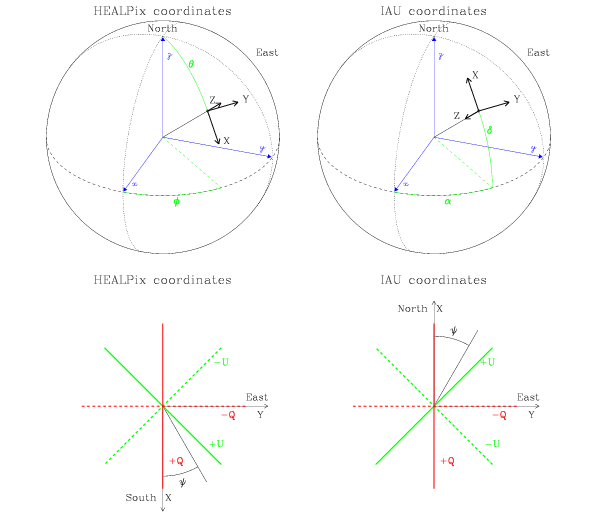
\includegraphics[bb=1pt 1pt 600pt 500pt,clip,width=0.95\textwidth]{fig/merge_reftqu.png}}
\latexhtml{%for latex
\centerline{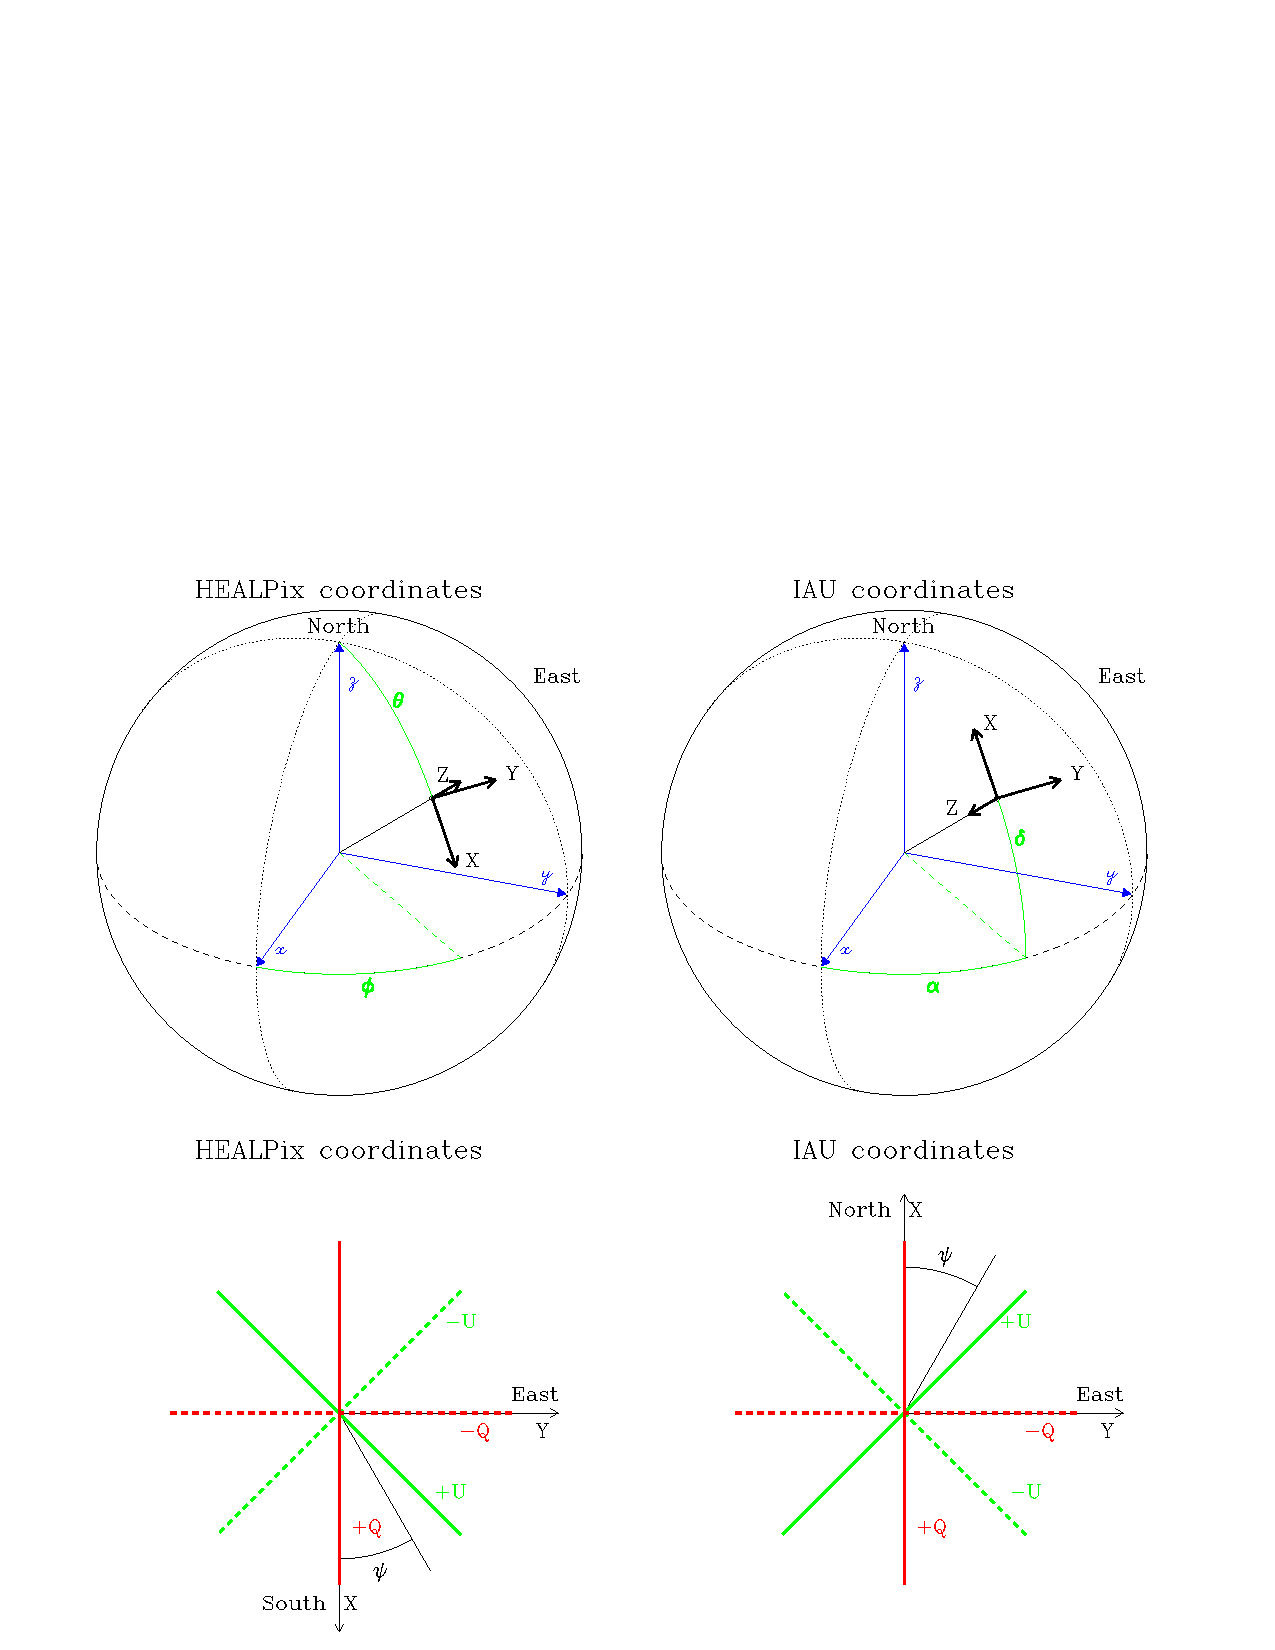
\includegraphics[clip,bb=0pt 0pt 600pt 520pt, width=0.99\textwidth,clip]{fig/merge_reftqu.pdf}}
}{%for html
%\centerline{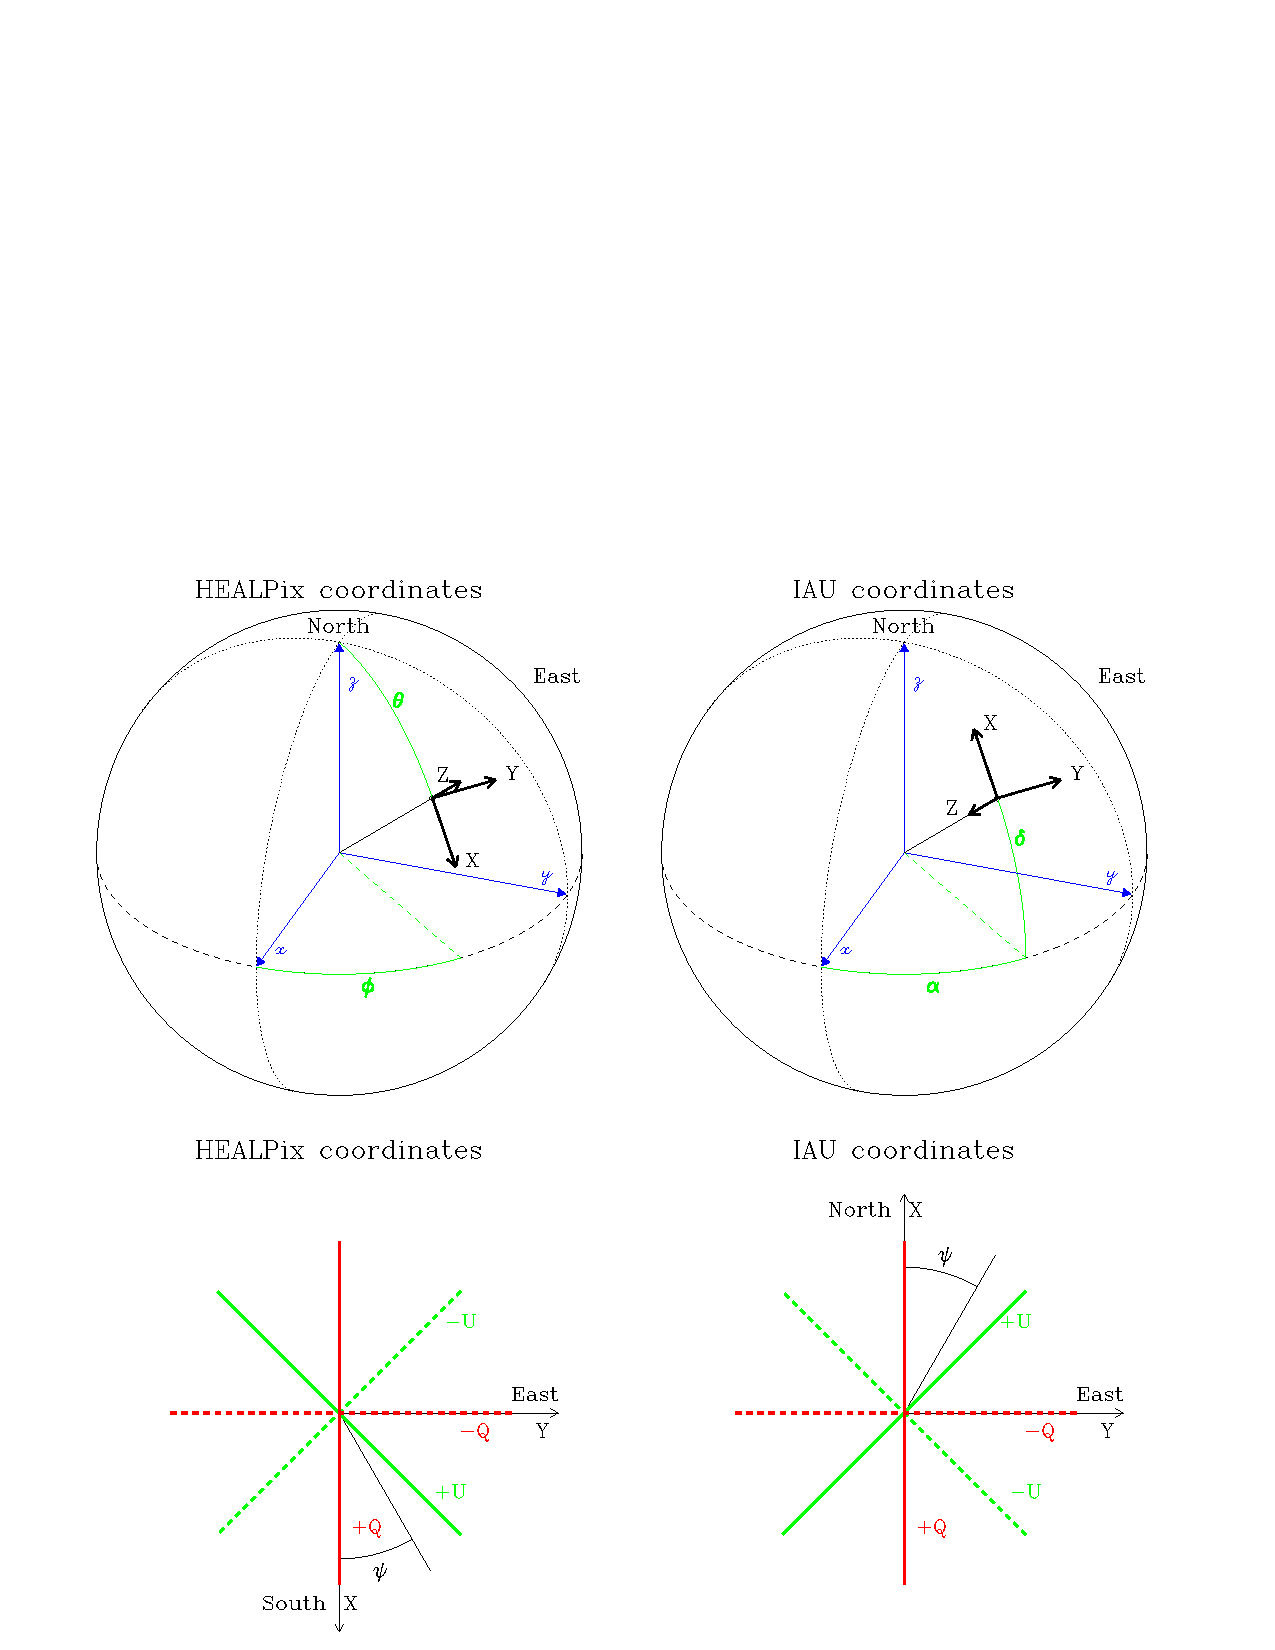
\includegraphics[bb=1pt 1pt 600pt520pt,clip,width=0.99\textwidth,clip]{fig/merge_reftqu}\htmlimage{}}
\centerline{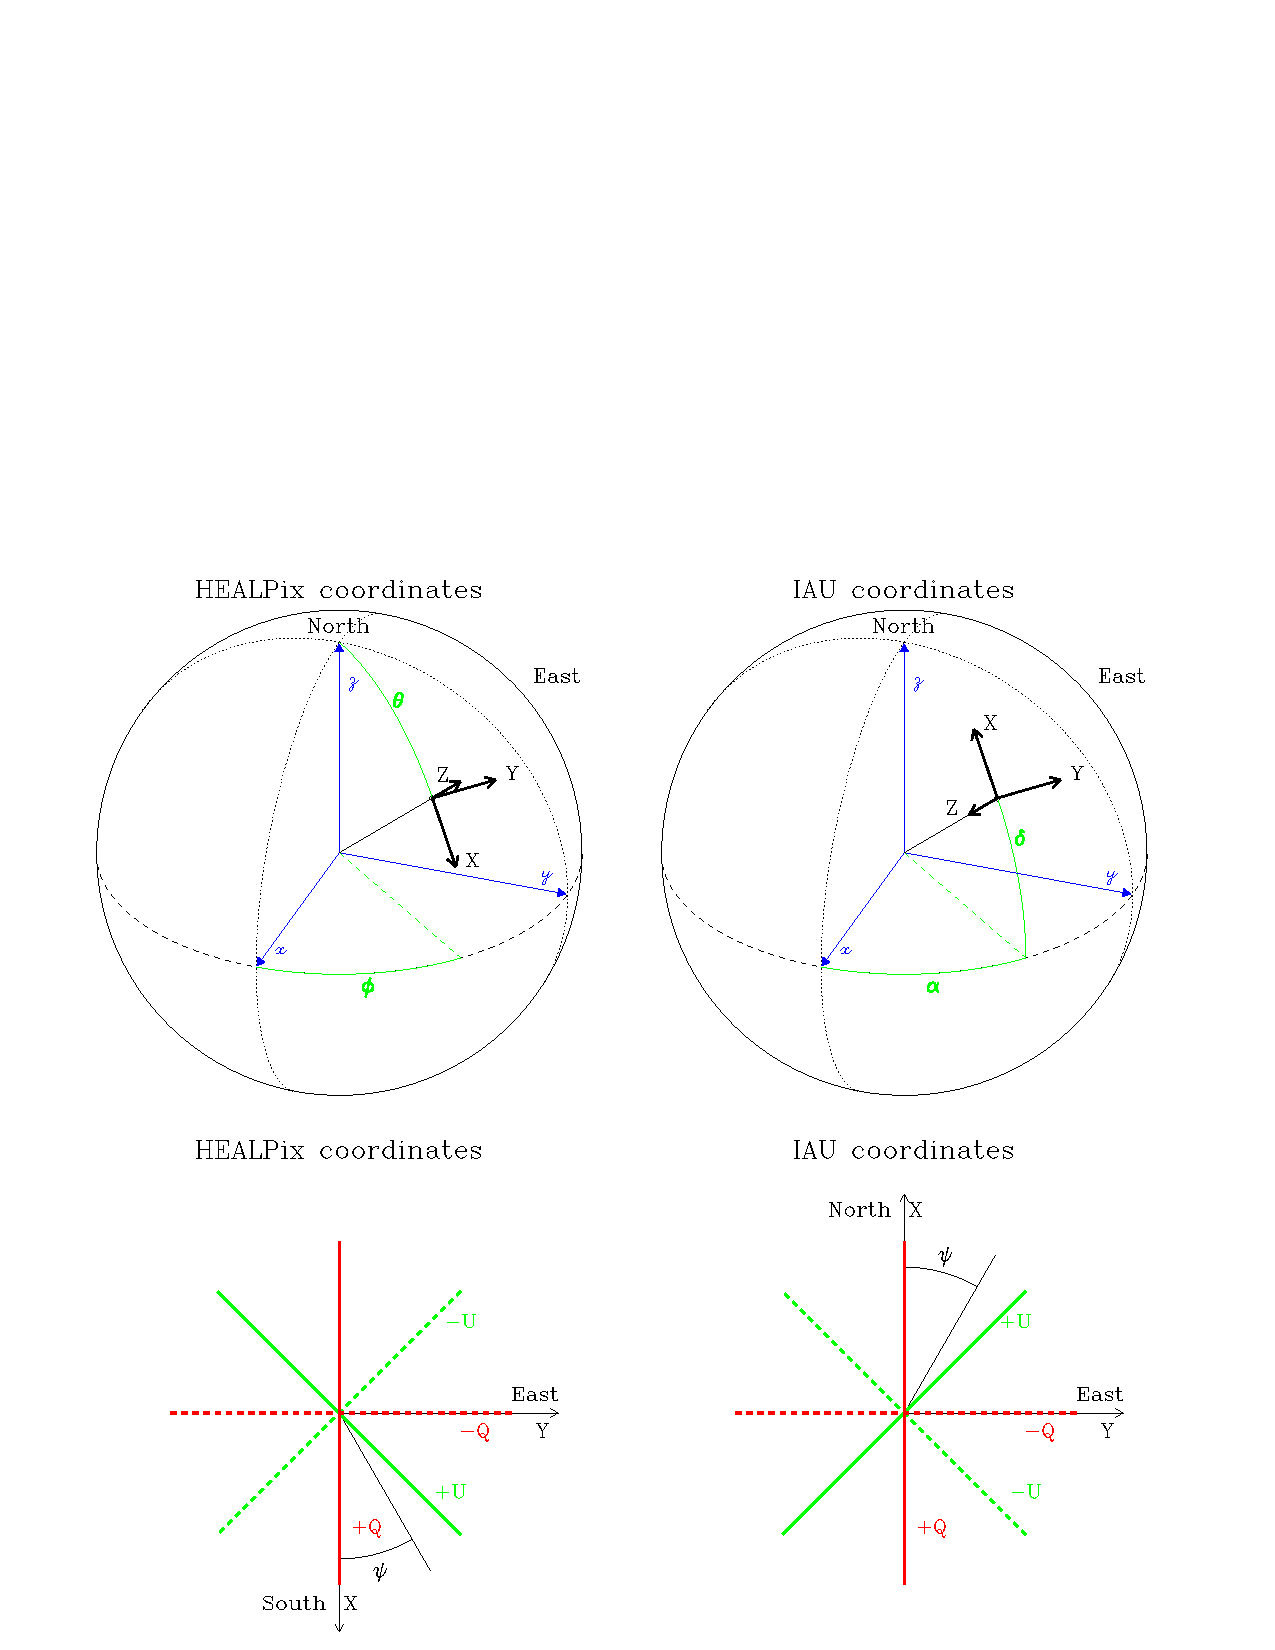
\includegraphics[width=\htmlfigwidth]{fig/merge_reftqu}}
}
\caption[Coordinate conventions]%
{\label{fig:reftqu}%
Coordinate conventions for \healpix ({\em lhs} panels) and IAU ({\em rhs} panels). The
  upper panels illustrate how the spherical coordinates are measured, and the
  lower panel how the $Q$ and $U$ Stokes parameters are identified in the
  tangential plan.
}
\end{figure}

The polarization conventions defined by the International Astronomical Union
\citep{iau74} are summarized in \cite{hambreg}. They define at each point on the
celestial sphere a cartesian referential with the $x$ and $y$ axes pointing
respectively toward the North and East, and the $z$
axis along the line of sight pointing toward the observer (ie, inwards) for a
right-handed system.

On the other hand, following the mathematical and CMB litterature tradition,
\healpix defines a cartesian referential with the $x$ and $y$ axes pointing
respectively toward the {\em South} and East, and the $z$ axis along the line of sight
pointing away from the observer (ie, {\em outwards}) for a right-handed
system. The {\em Planck} CMB mission follows the same convention \citep{ansari}.

The consequence of this definition discrepency is a change of sign of $U$,
which, if not accounted for, jeopardizes the calculation of the Electric and Magnetic  CMB
polarisation power spectra.

\vskip 0.3cm
\noindent{\bf{How \healpix deals with these discrepancies}}\\
The FITS keyword {\tt POLCCONV} has been introduced in \healpix 2.0 to describe the
polarisation coordinate convention applied to the data contained in the file. Its value is either {\tt
  COSMO} for files following the Healpix/CMB/{\em Planck} convention (default
for sky map synthetized with Healpix routine 
\htmlref{{\tt synfast}}{fac:synfast}
or {\tt IAU} for those
following the IAU convention, as defined above. Absence of this keyword is
interpreted as meaning {\tt COSMO}.

The \htmlref{{\tt change\_polcconv}}{idl:change_polcconv} IDL facility is provided to add this keyword or
change/update its value and swap the sign of the $U$ Stokes parameter, when applicable, in
an existing FITS file.

The facility \htmlref{{\tt anafast}}{fac:anafast} will crash if the map to analyze follows the 'IAU'
convention, and issue a warning if the convention used can not be determined.


%------------------------ P _ l _ m -------------------
%
\subsection{Spherical harmonic conventions}
%%\addcontentsline{toc}{subsection}{\numberline{}Some properties of spherical harmonics}
\label{sphericalstuff}

The Spherical Harmonics are defined as
\begin{eqnarray}
	Y_{\ell m}(\theta,\phi) &\myequal& \lambda_{\ell m}(\cos\theta) {\rm{ e}}^{{i}
	m\phi} \label{eq:ylm_def} \myhtmlimage{}
\end{eqnarray}
where the 
\begin{eqnarray}
	\lambda_{\ell m}(x) &\myequal& \sqrt{ \frac{2\ell+1}{4\pi}
	\frac{(\ell-m)!}{(\ell+m)!} } P_{\ell m}(x), \quad{\rm for~}
	m\ge 0 	\label{eq:lam_def} \\
%
	\lambda_{\ell m} &\myequal& (-1)^m \lambda_{\ell |m|}, \quad{\rm for~}
	m <  0, \nonumber \\
%
	\lambda_{\ell m} &\myequal& 0, \quad{\rm for}\, |m| > \ell.\nonumber
	\myhtmlimage{}
\end{eqnarray}

Introducing $x\equiv\cos\theta$, the associated Legendre Polynomials $P_{\ell m}$ 
solve the differential equation
\begin{eqnarray}
	(1-x^2)\frac{d^2}{dx^2}P_{\ell m} - 2x \frac{d}{dx}P_{\ell m}
	+ \left(\ell(\ell+1) - \frac{m^2}{1-x^2}\right) P_{\ell m} &\myequal& 0.
	\myhtmlimage{}
\label{eq:diff_eq}
\end{eqnarray}
They are related to the ordinary Legendre Polynomials $P_l$ by
\begin{eqnarray}
	P_{\ell m} &\myequal& (-1)^m (1-x^2)^{m/2} \frac{d^m}{dx^m} P_{\ell}(x),
	\myhtmlimage{}
\label{eq:legendreass}
\end{eqnarray}
which are given by the Rodrigues formula
\begin{eqnarray}
	P_{\ell}(x) &\myequal& \frac{1}{2^\ell \ell!}\frac{d^\ell}{dx^\ell} (x^2-1)^\ell.
	\myhtmlimage{}
\label{eq:rodrigues}
\end{eqnarray}

Note our $Y_{\ell m}$ are identical to those of \citet{edmonds},
even though our definition of the $P_{\ell m}$ differ from his by a factor
$(-1)^m$ ({\it a.k.a.} Condon-Shortley phase).

\section{Pixel window functions}
\renewcommand{\u}{{\bf{u}}}
%\warnhtml

A pixelated signal $f(p)$ is the average within each pixel $p$ (with surface
area $\Opix$) of the underlying signal 
\begin{eqnarray}
  f(p) &\myequal& \int d\u w_p(\u)f(\u) \myhtmlimage{}
\end{eqnarray}
where $w_p$ is equal to $1/\Opix$ within the pixel, and equal to 0 outside, so
that $\int d\u w_p(\u) = 1$.
Eq.~(\ref{eq:alms}) then becomes
\begin{eqnarray}
  f(p)&\myequal&\sum_{\ell =0}^{\ell_{max}}\sum_{m}a_{\ell m}w_{\ell m}(p),
\myhtmlimage{}
\end{eqnarray}
where
%% $\int d\u w_p(\u) = 1$
%% The effect of the finite pixel size on the measured power of a pixelated map
%% depends on the average of the Spherical Harmonic on pixel $p$ (of surface area $\Opix$), defined as
\begin{eqnarray}
 	w_{\ell m}(p) &\myequal& \int d\u w_p(\u) Y_{\ell m}(\u), \myhtmlimage{} \label{eq:pixel_lmp} 
\end{eqnarray}
is the Spherical Harmonic Transform of the pixel $p$.
%% where $w_p$ is equal to $1/\Opix$ within the pixel, and equal to 0 outside, such that
%% $\int d\u w_p(\u) = 1$.

However, complete analysis of a pixelated map with the exact $w_{\ell m}(p)$
defined above would be computationally intractable (because of azimutal
variation of pixel shape over the polar caps of the \healpix grid), 
and some simplifying asumptions have to be
made. If the pixel is small compared to the signal correlation length
(determined by the beam size), the exact structure of the pixel can be ignored
in the subsequent analysis and we can {\em assume}
\begin{eqnarray}
  w_{\ell m}(p) = w_\ell(p) Y_{\ell m}(p)\myhtmlimage{}
\end{eqnarray}
where we introduced the $m$-averaged window function
\begin{eqnarray}
	w_{\ell}(p) &\myequal& \left(\frac{4 \pi}{2\ell+1}\sum_{m=-\ell}^{\ell} \left|w_{\ell m}(p)\right|^2\right)^{1/2},\myhtmlimage{}
	\label{eq:pixel_lp} 
\end{eqnarray}
which is independent of the pixel location on the sky.

If we assume all the pixels to be identical, the power spectrum of the
pixelated map, $C_{\ell}^{\rm pix}$, is related to the hypothetical unpixelated
one, $C_{\ell}^{\rm unpix}$, by 
\begin{eqnarray}
	C_{\ell}^{\rm pix} &\myequal& w^2_{\ell} C_{\ell}^{\rm unpix} \myhtmlimage{}
	\label{eq:cl_pixel} 
\end{eqnarray}
where the effective pixel window function $w_{\ell}$ is defined as
\begin{eqnarray}
	w_{\ell} &\myequal& \left(\frac{1}{\npix}\sum_{p=0}^{\npix-1} w^2_{\ell}(p)\right)^{1/2}.\myhtmlimage{}
	\label{eq:pixel_l} 
\end{eqnarray}
This function is provided with the \healpix package for $\ell\le 4\nside$ for each
resolution parameter $\nside$.

The pixel window functions are now available for both temperature and
polarization.

For $\nside \le 128$, those window functions are computed exactly using
Eqs.~(\ref{eq:pixel_lp}) and (\ref{eq:pixel_l}). For $\nside > 128$ the
calculations are too costly to be done exactly at all $\ell$. The temperature
windows are
extrapolated from the case $\nside = 128$ assuming a scaling in $\ell$ similar
to the one exhibited by the window of a tophat pixel. The polarization
windows are assumed to be proportional to those for temperature, with a
proportionality factor given by the exact calculation of $w_{\ell}$ at low
$\ell$.

Because of a change of the extrapolation scheme used, the temperature window
functions provided with \healpix 1.2 and higher for $\nside > 128$ are slighty different from those
provided with \healpix 1.1. For a given $\nside$, the relative difference
increases almost linearly with $\ell$, and is of the order of $\Delta w/w < 7\ 10^{-4}$ at
$\ell=2\nside$ and $\Delta w/w < 1.7\ 10^{-3}$ at $\ell=4\nside$.

% We have checked that in the range $\ell < 1024$ and for the pixel size
% considered here (6.87 arcmin) the discrepency between the
% whole-sky average pixel window function $w_{\ell}$ and any individual one is an
% increasing function of $\ell$ which vanishes at low $\ell$ and is at most 5\% at
% $\ell = 1024$ for the worst case pixel. We also checked that
% in the region of the sky analyzed in this paper the average window
% differs by less than 1.2\% from the whole sky average.


\section{A Comment on the Random Number Generator}

We provide a new random number generator (RNG) with this package, available both
in Fortran90 and C++. 
It resides in {\tt src/f90/mod/rngmod.f90} and {\tt
  src/cxx/cxxsupport/planck\_rng.h} and supersedes the previous RNG (which
is still available at {\tt src/f90/mod/ran\_tools\_dist.f90}). 

It produces double precision real numbers $x$ with $x\in]0,1[$ and is based 
on a xorshift method described by Marsaglia in 
Journal of Statistical Software 2003, vol 8
(cf. \htmladdnormallink{{\tt http://www.cs.hku.hk/}}{http://www.cs.hku.hk/}).
It accepts up to four different seeds simultaneously, allowing each sequence to
have a
theoretical period of $2^{128}-1 \approx 3.4 10^{38}$. A Gaussian deviate RNG is
also provided. See the respective routines documentation for details on their usage.
Please note that we have not extensively tested this generator 
--- it did not represent the main drive of this project.

%% \section{Shortcut in calculation of the Spherical Harmonics}

%% and combines two pseudo-random numbers from simple 32 bit RNGs  
%% into one by addition modulo $2^{30}$. The two simple RNGs are a 2*16 bit
%% multiply-with-carry RNG and a Marsaglia shift register.
%% Please note that we have not extensively tested this generator 
%% --- it did not represent the main drive of this project.

%% From theoretical expectations this RNG should provide at least as good 
%% performance as the \$1000 guaranteed Numerical Recipes ``ran2'', but we are
%% not willing to enter any bets. Its calling interface is
%% identical to ``ran2'' and it should therefore be trivial to replace it
%% with the RNG of your choice.
\newpage

%\printindex

\bibliographystyle{apalike}
\begin{thebibliography}{99}
%
%%%\backrefparscanfalse

\bibitem[Ansari et al, 2003]{ansari}
Ansari, R., et al, 2003, {\em Planck parameter definition document} (DRAFT
2003-10-23), Technical Report PL-COM-IAS-SD-L2.02.005, ESA.
%
\bibitem[Baumgardner \& Frederickson (1985)]{baum}
Baumgardner, J.R. and Frederickson, P.O., 1985, SIAM J. Numerical Analysis, Vol. 22,
No. 6, p. 1107
%
\bibitem[Boch et al, 2014]{moc}
Boch, T., Donaldson, T., Durand, D., et al. 2014, 
``{\em MOC-HEALPix Multi-Order Coverage map}'', 
\htmladdnormallink{http://ivoa.net/documents/MOC/}{http://ivoa.net/documents/MOC/}

\bibitem[Chandrasekhar (1960)]{chandra}  
Chandrasekhar, S. 1960, in Radiative Transfer (Dover: New York) 

\bibitem[Chon et al (2004)]{polspice}
Chon, G., Challinor, A., Prunet, S., Hivon, E. \& Szapudi, I., 2004, 
\htmladdnormallink{MNRAS, 350, 914}{http://cdsads.u-strasbg.fr/abs/2004MNRAS.350..914C}.
PolSpice code available at \htmladdnormallink{http://www2.iap.fr/users/hivon/software/PolSpice/}{%
http://www2.iap.fr/users/hivon/software/PolSpice/}
%http://cdsads.u-strasbg.fr/abs/2004MNRAS.350..914C


%   eprint = {astro-ph/0303414},

\bibitem[Crittenden et al (1995)]{crco}
Crittenden, R.G., Coulson, D. \&  Turok, N.G., 1995, Phys.Rev. D52, 5402

\bibitem[Crittenden \& Turok (1998)]{crtu}
Crittenden, R. and Turok, N.G., 1998, \htmladdnormallink{astro-ph/9806374}{http://arXiv.org/abs/astro-ph/9806374}

\bibitem[Doroshkevich et al. (2005)]{glesp}
Doroshkevich, A.G.,
Naselsky,    P.D.,  
Verkhodanov, O.V.,  
Novikov,     D.I.,  
Turchaninov, V.I.,  
Novikov,     I.D.,  
Christensen, P.R. \&
Chiang,	     L.-Y., 2005,
IJMPD, 14, 2, 275, \htmladdnormallink{astro-ph/0305537}{http://arXiv.org/abs/astro-ph/0305537}

\bibitem[Driscoll \& Healy (1994)]{drhea}
Driscoll, J.R. and Healy, D., 1994, Adv. in Appl. Math., Vol. 15, p.202

\bibitem[Edmonds, 1957]{edmonds}
Edmonds, A.R., 1957, {\em Angular Momentum in Quantum Mechanics}, Princeton
University Press

\bibitem[Goldberg (1967)]{goldberg} 
Goldberg, J. N., et al. 1967, J. Math. Phys. 8, 2155

\bibitem[G{\'o}rski et al (2005)]{gorskihealpix05}
  G\'orski, K.M., Hivon, E., Banday, A.~J., Wandelt,
  B.~D., Hansen, F.~K., Reinecke, M. \& Bartelmann, M., 2005, 
\htmladdnormallink{ApJ, 622, 759}{http://adsabs.harvard.edu/cgi-bin/nph-bib_query?bibcode=2005ApJ...622..759G&amp;db_key=AST&amp;high=41069202cf02947}, 
\htmladdnormallink{astro-ph/0409513}{http://arxiv.org/abs/astro-ph/0409513}

\bibitem[Hamaker \& Bregman, 1996]{hambreg}
Hamaker, J.P. \& Bregman, J.D., 1996, A\&AS 117, 161

\bibitem[Hamaker \& Leahy, 2003]{hamakerleahy}
  Hamaker, J.P. \& Leahy, J.P., 2003, {\em ``A study of CMB differencing
  polarimetry with particular reference to {\em Planck}}'', {\sc ESA Report SCI-A/2003.312/jt}

\bibitem[Hivon et al (2002)]{master}
Hivon, E., G{\'o}rski, K, M., Netterfield, C. B., Crill, B. P., Prunet, S. \& Hansen, F., 
2002, \htmladdnormallink{ApJ, 567, 2}{http://cdsads.u-strasbg.fr/abs/2002ApJ...567....2H}, 
\htmladdnormallink{astro-ph/0105302}{http://arxiv.org/abs/astro-ph/0105302}

\bibitem[Hu \& White (1997)]{primer}
Hu, W. \& White, M., 1997, NewA, 2, 323

\bibitem[IAU, 1974]{iau74}
IAU, 1974, Transactions of the IAU Vol. 15B (1973) 166

\bibitem[Kamionkowski et al (1997)]{kks}
Kamionkowski, M., Kosowsky, A., Stebbins, A., 1997, Ph.Rev. D, 55, 7368 (KKS)

\bibitem[Muciaccia, Natoli \& Vittorio (1998)]{munavi}
Mucaccia, P.F, Natoli, P. and Vittorio, N., 1998, ApJ, 488, L63

\bibitem[Planck 2015-XI (2015)]{planck2015-11}
Planck Collaboration, 2015-XI, \htmladdnormallink{arXiv:1507.02704v1}{http://arXiv.org/abs/1507.02704v1}

\bibitem[Reinecke \& Hivon, 2015]{rh15}
Reinecke, M. and Hivon, E., 2015, 
\htmladdnormallink{A\&A, 580, A132}{http://cdsads.u-strasbg.fr/abs/2015A\%26A...580A.132R}, 
\htmladdnormallink{arXiv:1505.04632v2}{http://arxiv.org/abs/1505.04632}

\bibitem[Rocha et al, 2009]{xfaster}
Rocha, G., Contaldi, C.R., Bond, J.R. \& G\'orski, K.M., 2009,
\htmladdnormallink{arXiv:0912.4059v2}{http://arxiv.org/abs/0912.4059}

\bibitem[Saff \& Kuijlaars (1997)]{mathint}
Saff, E.B. and Kuijlaars, A.B.J., 1997, The Mathematical 
Intelligencer, 19, \#1, p.5

\bibitem[Seljak \& Zaldarriaga (1997)]{longspin}
Seljak, U. \& Zaldarriaga, M., Phys. Rev. Lett. {\bf 78}, 2054 (1997).   

\bibitem[Szalay \& Brunner (1998)]{szalay}
Szalay, A.S. and Brunner, R.J., 1998, 
\htmladdnormallink{astro-ph/9812335}{http://arXiv.org/abs/astro-ph/9812335}, to appear in 
a special issue of the Elsevier journal "Future Generation Computer Systems"

\bibitem[Tegmark (1996)]{teg}
Tegmark, M., 1996, ApJ, 470, L81

\bibitem[Tristram et al (2005)]{xspect}
Tristram, M., Macias-Perez, J.F., Renault, C., \& Santos, D., 2005, 
\htmladdnormallink{MNRAS, 358, 833}{http://cdsads.u-strasbg.fr/abs/2005MNRAS.358..833T}

\bibitem[Wandelt, Hivon \& G\'orski (1998)]{whg}
Wandelt, B.D., Hivon, E. and G\'orski, K.M., 1998, 
\htmladdnormallink{astro-ph/9803317}{http://arXiv.org/abs/astro-ph/9803317}, in
 "Fundamental Parameters in Cosmology", proceedings of the XXXIIIrd Rencontres
de Moriond, Tr{\^a}n Thanh V{\^a}n (ed.)

\bibitem[Wandelt, Hivon \& G\'orski (2001)]{whg2001}
Wandelt, B.D., Hivon, E. and G\'orski, K.M., 2001, 
\htmladdnormallink{Phys. Rev. D, 64, 083003}{http://adsabs.harvard.edu/abs/2001PhRvD..64h3003W},
\htmladdnormallink{astro-ph/9808292v1}{http://arXiv.org/abs/astro-ph/9808292v1}

%% \bibitem{fastah} Wandelt, B.D., G\'orski, K.M., Hivon, E.\ and Hansen,
%% F.\, in preparation
 
\bibitem[Zaldarriaga (1998)]{zalda} 
Zaldarriaga, M., 1998, ApJ, 503, 1

\bibitem[Zaldarriaga~\&~Seljak (1997)]{spinlong}
Zaldarriaga, M. \& Seljak, U., Phys. Rev. D {\bf 55} 1830 (1997)

%% \backrefprint\backrefparscantrue

\end{thebibliography}

\end{document}%%%%%%===================

